\documentclass[11pt,a4paper]{article}
\pdfoutput=1
\usepackage{jheppub}
\bibliographystyle{JHEP}
\usepackage{bm}
\usepackage{graphicx}
%\usepackage{afterpage}
\usepackage{mathtools}
\usepackage{mathrsfs}
\usepackage{subfigure}
\usepackage[svgnames]{xcolor}
\usepackage{slashed}
%\usepackage[caption=false]{subfig}
%\usepackage[svgnames]{xcolor}
\usepackage{enumerate}
\usepackage{xspace}

\newcommand{\be}{\begin{equation}}
\newcommand{\ee}{\end{equation}}
\newcommand{\bq}{\begin{eqnarray}}
\newcommand{\eq}{\end{eqnarray}}
\newcommand{\one}{1 \!\! 1}
\newcommand{\D}{\mathrm{d}}
\newcommand{\E}{\mathrm{e}}
\newcommand{\I}{\mathrm{i}}
\def\Vec#1{\mathpalette{\VVec}{#1}}
\def\VVec#1#2{\mbox{\boldmath$#1#2$\unboldmath}}
\newcommand{\xbj}{\mathrm{x_{B}}}

\setcounter{page}{0}
%{CLAS Analysis Note XXXX}
\vskip1.5cm

\title{ Back-to-back prduction of hadrons in SIDIS} 
\author[a]{H. Avakian,}
\author[b]{M. Mirazita,}
\author[b]{S. Pisano,}
\author[c]{A. Kotzinian,}

\affiliation[a]{Thomas Jefferson National Accelerator Facility, Newport News, Virginia 23606, USA}
\affiliation[b]{INFN, Laboratori Nazionali di Frascati, 00044 Frascati, Italy}
\affiliation[c]{YerPHI, Yerevan Physics Institute, Armenia}

\emailAdd{avakian@jlab.org}
\emailAdd{marco.mirazita@lnf.infn.it}
\emailAdd{pisanos@lnf.infn.it}
\emailAdd{kotzinian@cern.ch}

\arxivnumber{JLAB-THY-XX-XXXX}

\abstract{
We report first measurements of the spin azimuthal asymmetries in
back-to-back hadron electroproduction in deep inelastic scattering kinematics
using a 5.7 GeV electron beam and the CEBAF Large Acceptance
Spectrometer (CLAS) at JLab.
Scattering of  longitudinally polarized electrons off unpolarized hydrogen targets was
studied over a wide range of kinematics.
Kinematic dependencies of single spin asymmetries
have been studied.
Non-zero $\sin\Delta\phi$ moments for $ep\rightarrow p\pi^+X$, where the $\Delta\phi$ is the difference of azimuthal angles of proton and pion in 
the CM frame, 
indicate that spin-orbit correlations between target and current fragments may be significant.
The dependence of the modulation on the product of transverse momenta of two hadrons is consistent with predictions based on fracture function formalism.
}
\keywords{SIDIS, parton intrinsic transverse momentum, azimuthal moments}


\begin{document}

\maketitle


\section{Introduction}

Understanding of the three-dimensional spin-dependent partonic structure of the nucleon, requires a full understanding of the hadronization 
process after the hard scattering.
Hadrons in hard scattering are produced from struck quark or in the current fragmentation region (CFR) as well as from target gragments, 
in the target fragmentation region (TFR).
The corresponding theoretical basis to study the TFR, based on  the fracture functions formalism, was established in Ref.~\cite{Trentadue:1993ka}
for hadron transverse momentum integrated unpolarized cross-section. Recently this approach was generalized~\cite{Anselmino:2011ss} to the spin and transverse momentum dependent case (STMD).

In electroproduction,
the polarized lepton emits a virtual photon with non--zero
longitudinal polarization,
which in turn selects preferentially one polarization state of the struck
quark. The opposite polarization and transverse momentum of a remnant $\bar{q}q$
pair can introduce correlations between  final--state $p,n,\Lambda,..$ hadrons produced 
in the target fragmentation region and hadrons produced in the current fragmentation.

Recently the leading twist formalism for spin and transverse-momentum dependent fracture functions has been  developed~\cite{Anselmino:2011ss}. 
The production of two hadrons in polarized SIDIS, with one spinless hadron produced in the current fragmentation region (CFR) and another in the TFR, would  provide access to the full set of leading twist fracture functions~\cite{Anselmino:2011bb}.


In the valence-quark region ($x > 0.1$) accessible at JLab
with CLAS at 5.7 GeV 
the polarization transfer from the beam is expected to be significant.
High luminosity
and high polarization of the electron beam makes CLAS
an ideal place for studies of correlations between target and current fragmentation regions.

%

In case of double hadron production process $l(\ell) + N(P) \to l(\ell') + h_1(P_1) + h_2(P_2) + X$,
al leading order LO, the cross-section includes all fracture functions~\cite{Anselmino:2011ss,Anselmino:2011bb}:
%
\bq \label{cs-2h}
&& \hspace{1.cm}
\frac{\D\sigma^{l(\ell,\lambda)+N(P,S) \to l(\ell')+h_1(P_1)+h_2(P_2)+X}}
{\D x \, \D y \, \D z_1 \, \D\zeta_2 \, \D^2 {\Vec P_{1\perp}} \,
\D^2 {\Vec P_{2\perp}} \, \D \phi_S} =
%\nonumber
\nonumber \\
&& \hspace{-0.2cm}
%\hspace{-1.cm}
\frac{\alpha^2\,x_B}{Q^4 \, y}\left[ 1+(1-y)^2 \right]
\left(\sigma_{UU} + S_\parallel \,\sigma_{UL} + S_\perp \,\sigma_{UT}+
\lambda \, D_{ll} \, \sigma_{LU} + \lambda \,S_\parallel D_{ll}\,\sigma_{LL}
+\lambda \, S_\perp D_{ll}\,\sigma_{LT} \right)\, ,
\nonumber
\eq
where $D_{ll}(y) = {y(2-y)}/{1+(1-y)^2}$ .
The subscripts in the structure functions $\sigma_{UT,UL,LT}$, specify the beam 
(first index) and  target (second index) polarization ($U,L,T$ for unpolarized, 
longitudinally and transversely polarized targets, and $U,L$ for unpolarized and 
longitudinally polarized beam).


\begin{table}[h]
\begin{center}
\caption{TABLE of Leading Twist FFs}
\vspace{0.2 truecm}
\begin{tabular}{|c|c|c|c|}
\hline
&$U$&$L$&$T$\\
\hline
$U$&$\hat{u}_1$&$\hat{l}^{\perp h}_1$&$\hat{t}^{h}_1,\hat{t}^{\perp }_1$ \\
\hline
$L$&$\hat{u}^{\perp h}_{1L}$&$\hat{l}_{1L}$&$\hat{t}^{h}_{1L},\hat{t}^{\perp }_{1L}$\\
\hline
$T$&$\hat{u}^{h}_{1T},\hat{u}^{\perp }_{1T}$&$\hat{l}^{h}_{1T},\hat{l}^{\perp }_{1T}$&$\hat{t}_{1T},\hat{t}^{hh}_{1T},\hat{t}^{\perp h}_{1T},\hat{t}^{\perp \perp }_{1T}$\\
\hline
\end{tabular}
\end{center}
\end{table}

Fo an unpolarized target expressions there are two contributions $\sigma_{UU}$ and $\sigma_{LU}$ ~\cite{Anselmino:2011ss}:
%
\bq\label{s_uu}
\sigma_{UU}  =  F_0^{{\hat u} \cdot D_1}
& - & D_{{nn}} \Bigg[\frac{P_{{1\perp}}^2 }{m_1 m_N}\, F_{{kp1}}^{{\hat t}^\perp \cdot H_1^\perp}\,{\cos}(2 \phi _1)
+ \frac{P_{{1\perp}} P_{{2\perp}} }{m_1 m_2}\, F_{{p1}}^{{\hat t}^h
\cdot H_1^\perp}\, {\cos}(\phi _1+\phi _2)\nonumber \\
& + & \left(\frac{P_{{2\perp}}^2 }{m_1 m_N}\, F_{{kp2}}^{{\hat t}^\perp
\cdot H_1^\perp} + \frac{P_{{2\perp}}^2 }{m_1 m_2}\, F_{{p2}}^{{\hat t^h}
\cdot H_1^\perp}\right)\, {\cos}(2 \phi _2)\Bigg].
\eq
\be
\sigma_{LU} = -\frac{ P_{{1\perp}} P_{{2\perp}}}{m_2 m_N}  F_{{k1}}^{{\hat l}^{\perp h}\cdot D_1} \, \sin(\phi _1-\phi _2)
\, ,
\ee

where the structure functions $F_{...}^{...}$ are specific convolutions~\cite{Anselmino:2011bb} of fracture and fragmentation functions depending on $x, z_1, \zeta_2, P_{1\perp}^2,  P_{2\perp}^2, {\Vec P}_{1\perp} \cdot
{\Vec P}_{2\perp}$.
The hadron 1 produced in the CFR ($x_{F1}>0$) is decribed by  standard scaled variable $z_1 \simeq P{\cdot}P_1/P{\cdot}q$,  and its transverse momentum ${\Vec P}_{1\perp}$ (with magnitude $P_{1\perp}$ and azimuthal angle
$\phi_1$) and the hadron 2, $h_2$  in the TFR ($x_{F2}<0)$ is decribed by similar variables,  $\zeta_2 \simeq E_2/E$
and ${\Vec P}_{2\perp}$ ($P_{2\perp}$ and $\phi_2$).


Large single-beam SSAs  for longitudinally polarized beam and one or two hadrons detected in the CFR have been observed at JLab \cite{Avakian:2003pk,E12-06-112B} and
HERMES~ \cite{Airapetian:2006rx}, which have been interpreted in terms of higher twist contributions, related to quark-gluon correlations.

The Target Fragmentation Region
(TFR) of DIS, which also carries interesting information about the spin and flavor structure
of the nucleon has not been studied systematically in experiments.The main physical question in the TFR is how the diquark-like remnant system after
the DIS process dresses itself up to become a full-fledged hadron, i.e., by which mechanism
the quark-antiquark pairs restoring color neutrality are produced, and how this process is
correlated with the spin of the target or/and the produced particles. In electroproduction, the
polarized lepton emits a virtual photon with non–zero longitudinal polarization, which in turn
selects preferentially one polarization state of the struck quark. The opposite polarization
of a remnant $s\bar{s}$ pair can again be transferred to the final–state  $\Lambda$  polarization, with the
efficiency extracted from eN collisions. After removing a polarized scattered quark from
an unpolarized nucleon, the remnant diquark may combine with an s quark, which could
originate from the nucleon sea or from a color string between the diquark and the scattered
quark to form a  $\Lambda$  hyperon. Significant polarization effects ($\sim$ 15−20\%) have been predicted in Intrinsic Strangeness Model (ISM) for  $\Lambda$  production in the TFR in deep-inelastic scattering  \cite{Ellis:1995fc}.
Longitudinal $\Lambda$ polarization transfer coefficient as a function of $x_F$ has been already 
measured with 5.5 GeV electron beam at CLAS (e1f data set). In Fig. \ref{fig:lambda12}, 
the measured asymmetry is  shown with the projected results for the future measurements using the CLAS12 detector and 11 GeV beam~\cite{E12-06-112A},  compared with the  ISM predictions  \cite{Ellis:1995fc}.

\begin{figure}
\begin{minipage}{.6\textwidth}
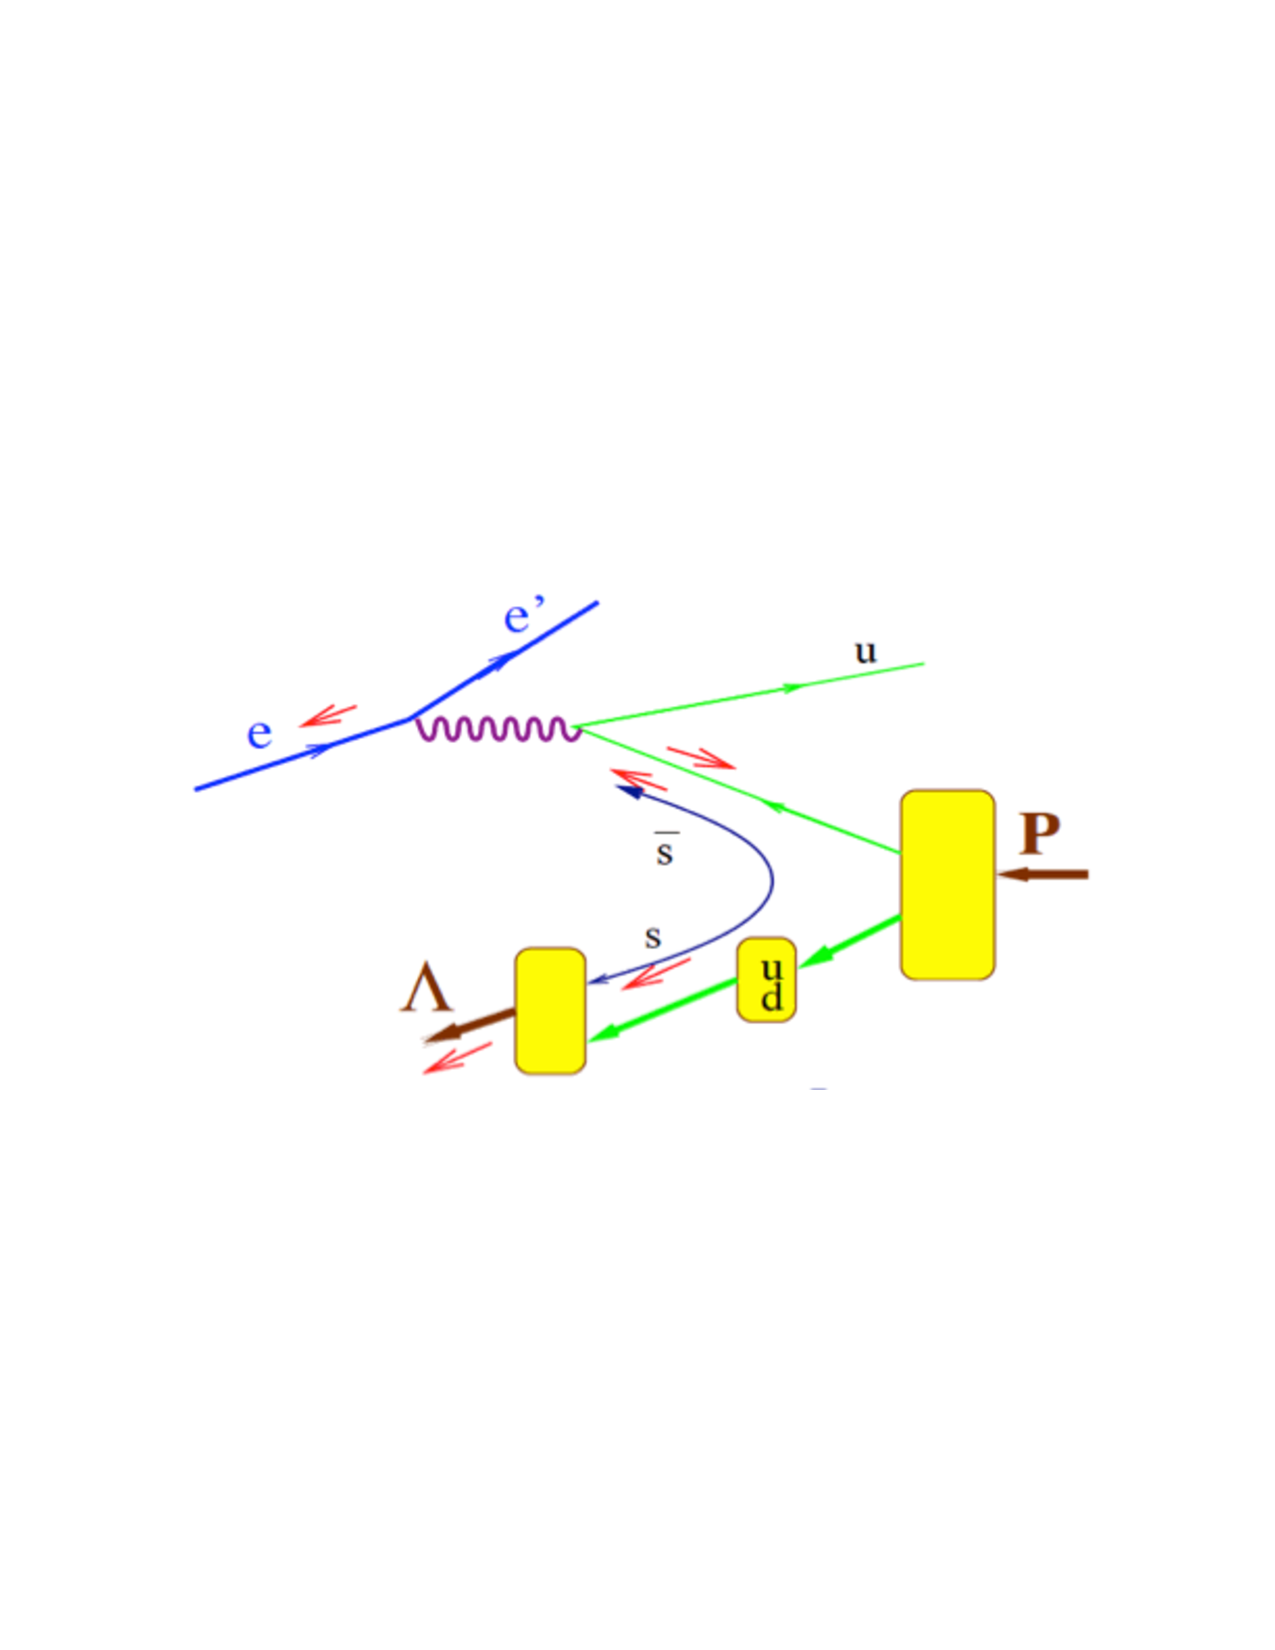
\includegraphics[width=8cm]{plots/lamdakin2.pdf}
\end{minipage}
\begin{minipage}{.6\textwidth}
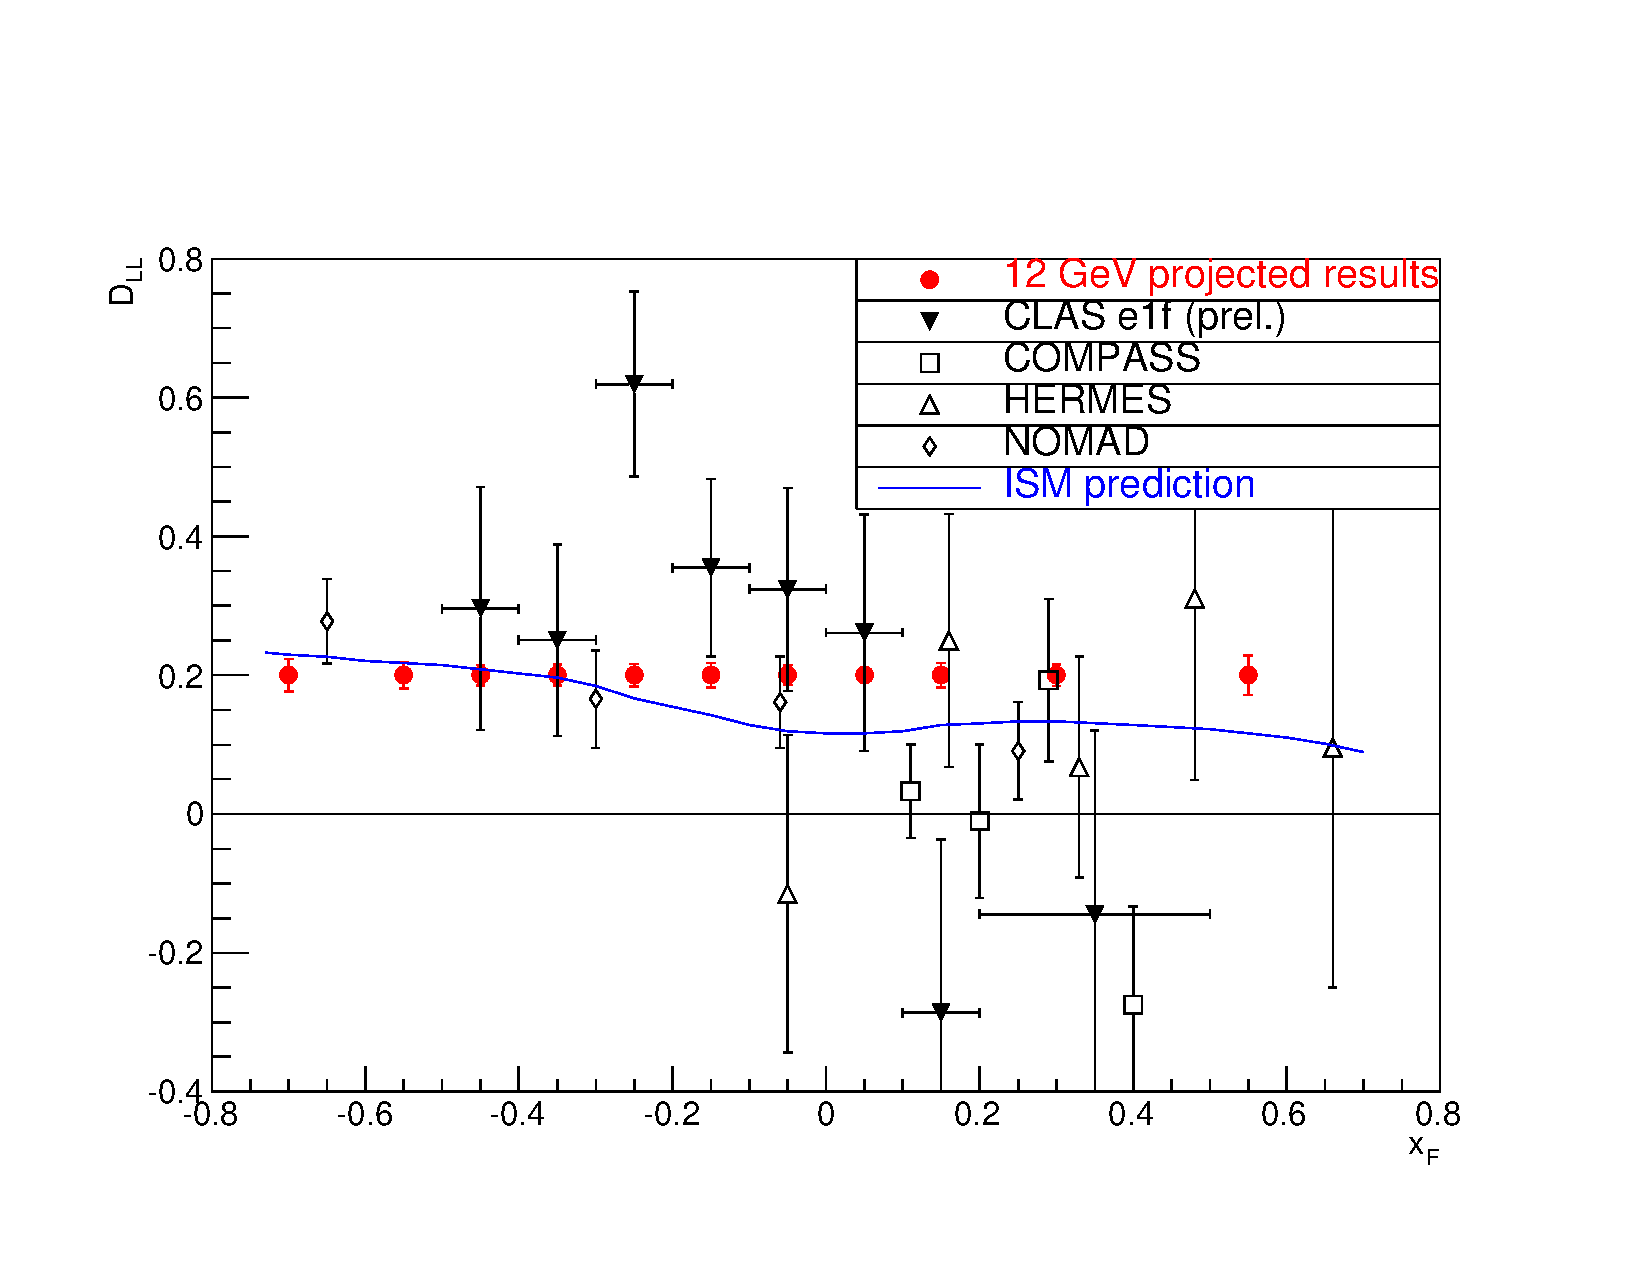
\includegraphics[width=8cm,height=6cm,keepaspectratio]{plots/lam-vs-xf-clas12.pdf}
\end{minipage}
   \caption{Dominant diagram for $\Lambda$  production in the target fragmentation region due to
scattering on a valence u quark (left) and Longitudinal $\Lambda$ polarization transfer coefficient as a function of $x_F$ from CLAS 5.49 GeV e1f data set (right).}
 \label{fig:lambda12}
 \end{figure} 


With hadrons detected in the TFR, the  beam  SSAs appear already at leading order.
With two hadrons detected in the final state, structure functions may depend also on the relative azimuthal angle of the two hadrons, 
generating a long range correlation between hadrons produced in CFR and TFR. 
The kinematic plane for back-to-back hadron production is shown on Fig. \ref{fig:b2b}.

\begin{figure}
\centering
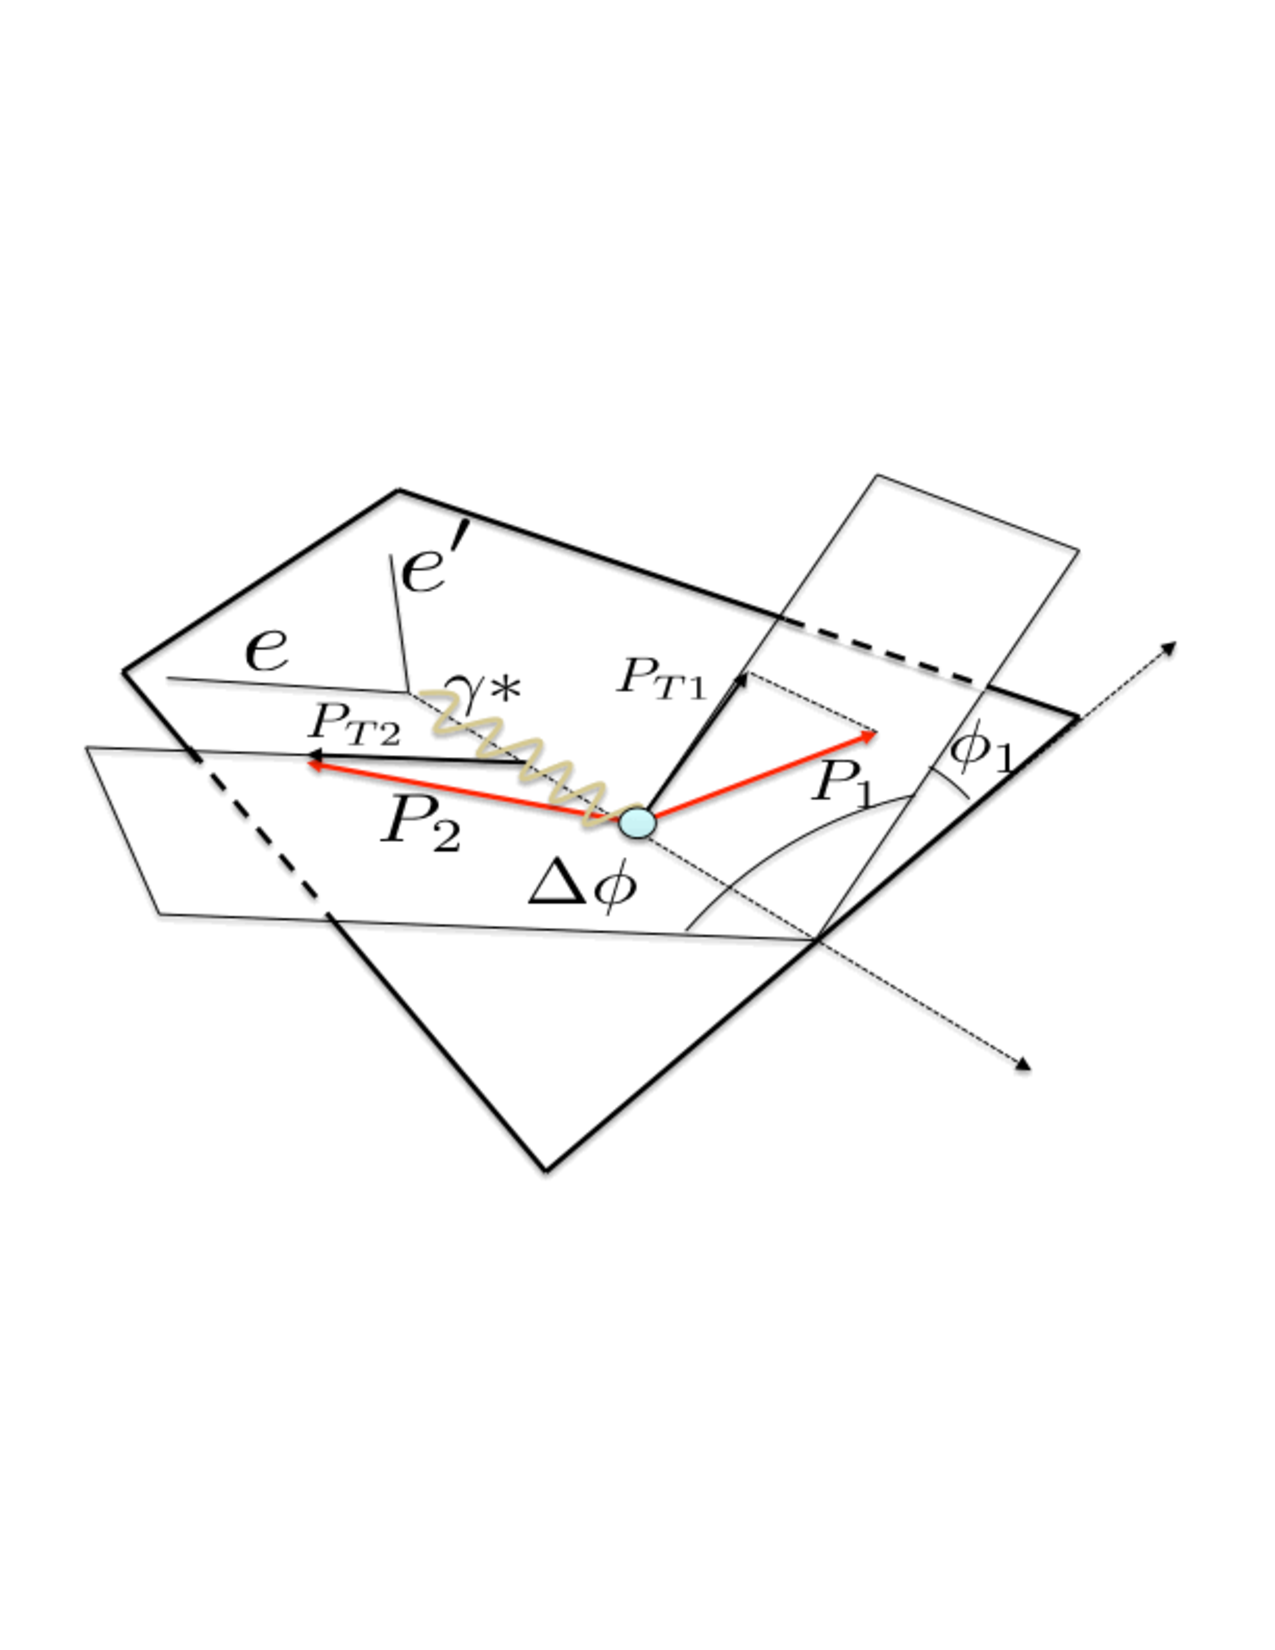
\includegraphics[width=16cm,height=10cm,keepaspectratio]{plots/b2bkin.pdf}
   \caption{Kinematic plane for back-to-back (b2b) hadron production in SIDIS}
 \label{fig:b2b}
 \end{figure} 


Choosing as independent azimuthal angles $\Delta \phi=\phi_2-\phi_1$ and $\phi_2$, the beam spin asymmetry could be defined as
\be
A_{LU}(x, z_1, \zeta_2, P_{1\perp}^2,  P_{2\perp}^2, \Delta \phi) =
\frac{\int \D \phi_2 \, \sigma_{LU}}{\int \D \phi_2 \, \sigma_{UU}}=
\frac{-\frac{ P_{{1\perp}} P_{{2\perp}}}{m_2 m_N}  F_{{k1}}^{{\hat l}^{\perp h}\cdot D_1} \, \sin(\Delta \phi)}{F_0^{{\hat u} \cdot D_1}}\,\cdot
\ee


Fracture functions can be modeled in different partonic models, which were used
to prdict  polarization of $\Lambda$ hyperons in the target fragmentation
region of DIS. The meson cloud model
\cite{Melnitchouk:1995en}, due to the pseudoscalar nature of the $N K \Lambda$ coupling,
predicts the polarization of final-state $\Lambda$ hyperons to be
strongly anticorrelated to that of the nucleon, vanishing for an
unpolarized target.

Large polarization effects ($\sim 15-20\%$) 
have been predicted in intrinsic strangeness model for $\Lambda$
production in the target fragmentation region in deep-inelastic
scattering \cite{Alberg:1995zp,Ellis:1994ww}.
Additional longitudinal polarization of the struck quark 
and remnant $s$ quark could be generated by the 
target polarization \cite{Ellis:1995fc}.
The sign of the polarization of $\Lambda$ hyperons produced in 
the DIS of polarized
charged-lepton off unpolarized nucleon depends on the sign of the
beam polarization and was predicted to be negative for the positive
lepton helicity. The spin transfer, is proportional to the
beam polarization, $P_B$, and the depolarization factor, $D(y)$.

\section{The Experiment}

This contribution presents measurements of
single spin asymmetries  in semi-inclusive productio of protons and charged pions in coincidence with the scattered electron in hard scattering kinematics  using a 5.7 GeV
electron beam and the CEBAF Large Acceptance 
Spectrometer (CLAS) \cite{Mecking:2003zu} at JLab.
Scattering of  longitudinally polarized electrons off
a 5-cm-long liquid-hydrogen target (e16 and e1f experiments) was 
studied over a wide range of kinematics.
The scattered electrons and photons were detected in
CLAS \cite{Mecking:2003zu}. The e16 and e1f data sets corresponds to an integral 
luminosity of $2.6\times 10^{40} cm^{-2}$ and  $3.1\times 10^{40} cm^{-2}$ respectively. 
The total number of events   
in the DIS range ($Q^2>1$ GeV$^2$, $W^2>4$ GeV$^2$)
selected by  quality, vertex, acceptance, fiducial, and kinematic cuts 
was $\approx 8\times 10^6$ for electron-proton coincidences.
The relative kinematic coverage of two data sets is shown in Fig. \ref{fig:xvsq2.e1fe16bins}.

\begin{figure}
\centering
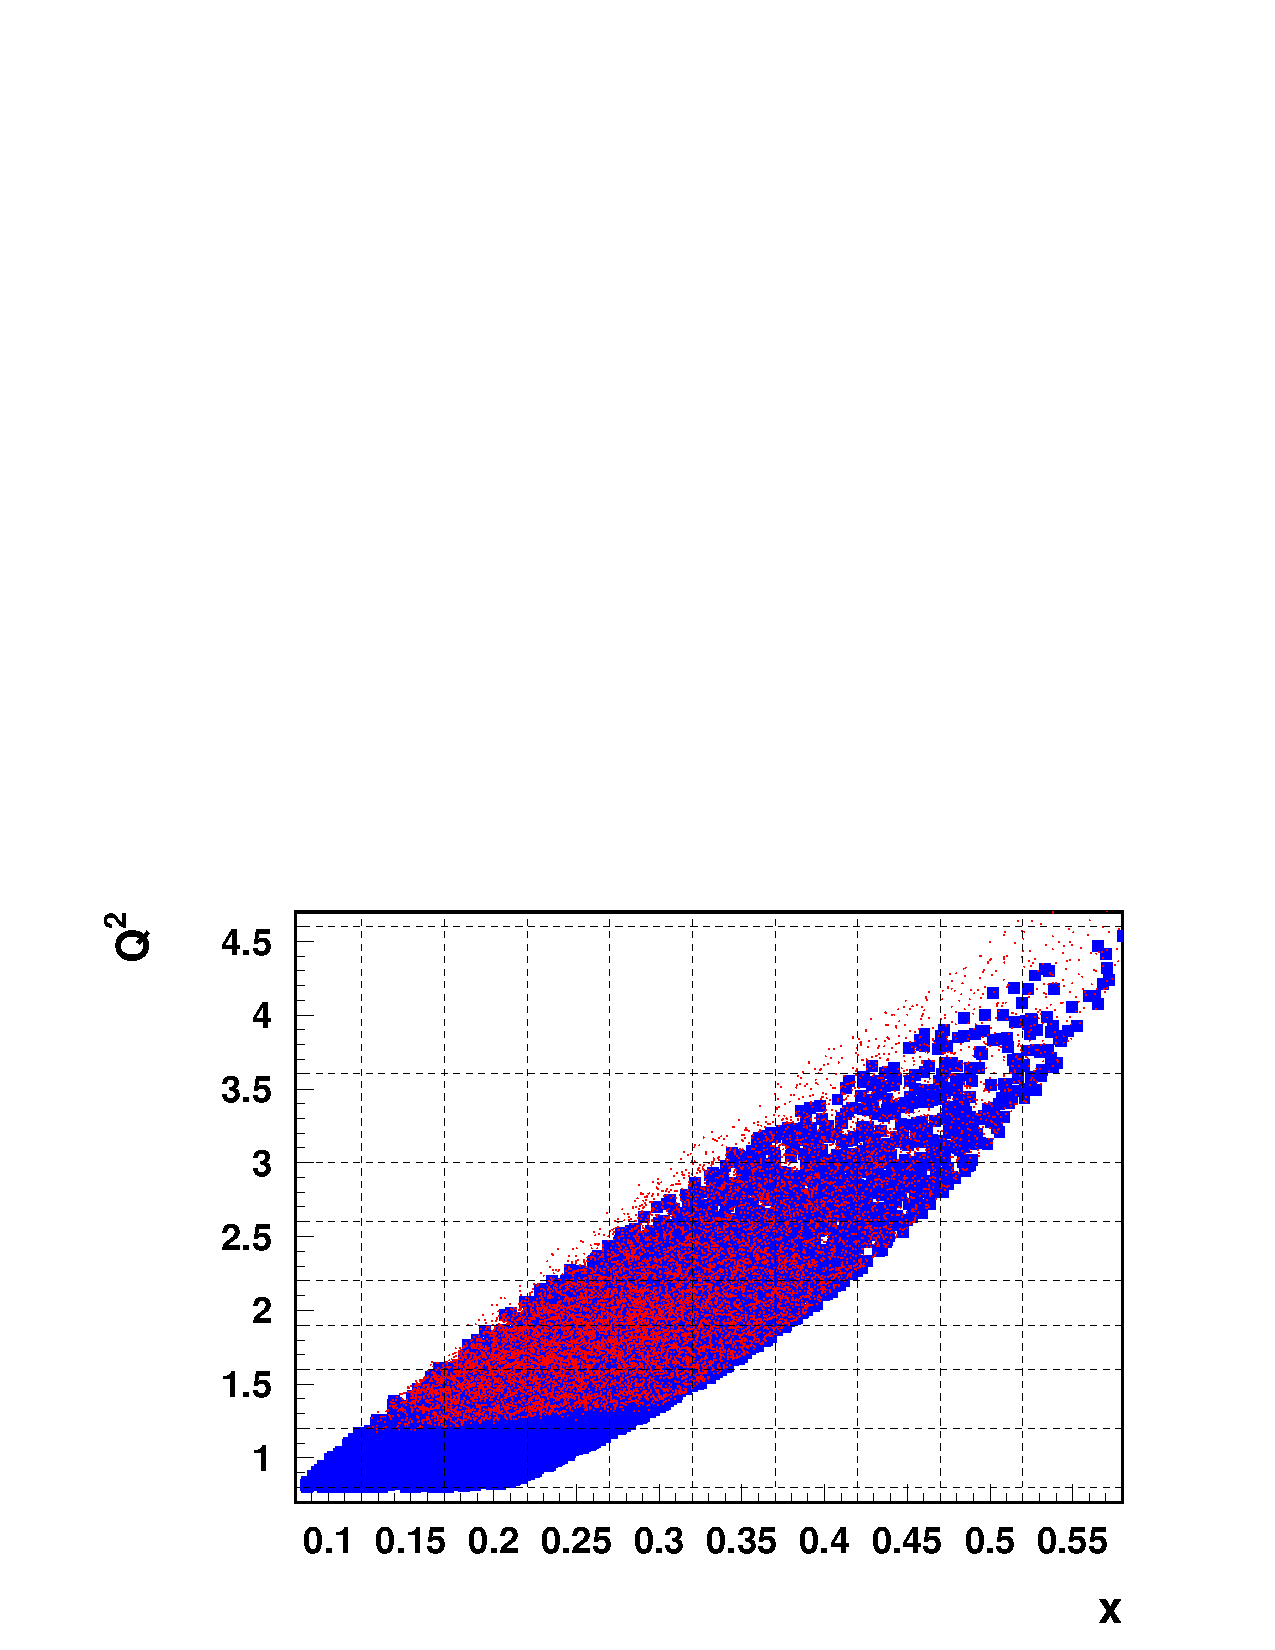
\includegraphics[width=0.8\textwidth]{plots/xvsq2-e1fe16bins.pdf}
   \caption{ Kinematic coverage in  $Q^2$ vs $x$ for e1f(blue squares) and e16 (red dots) 
data sets.}
 \label{fig:xvsq2.e1fe16bins}
 \end{figure} 


Extensive MC studies were performed
to define the fiducial and particle identification cuts. Tighter fiducial
cuts on pion variables were applied to the  sample to reduce the background from
other channels significantly.



\section{Data Quality}

\subsection{Binning}
The Fig. \ref{fig:e16bins} shows the binning of the $ep\pi^+$ event sample. 


\subsection{Fiducial and vertex cuts}

For the $ep$ sample Standard fiducial cuts were applied to restrict the kinematics to region,
where CLAS acceptance and efficiency is well under control 
(see Fig. \ref{fig:e16thvsphi})
\begin{figure}
\centering
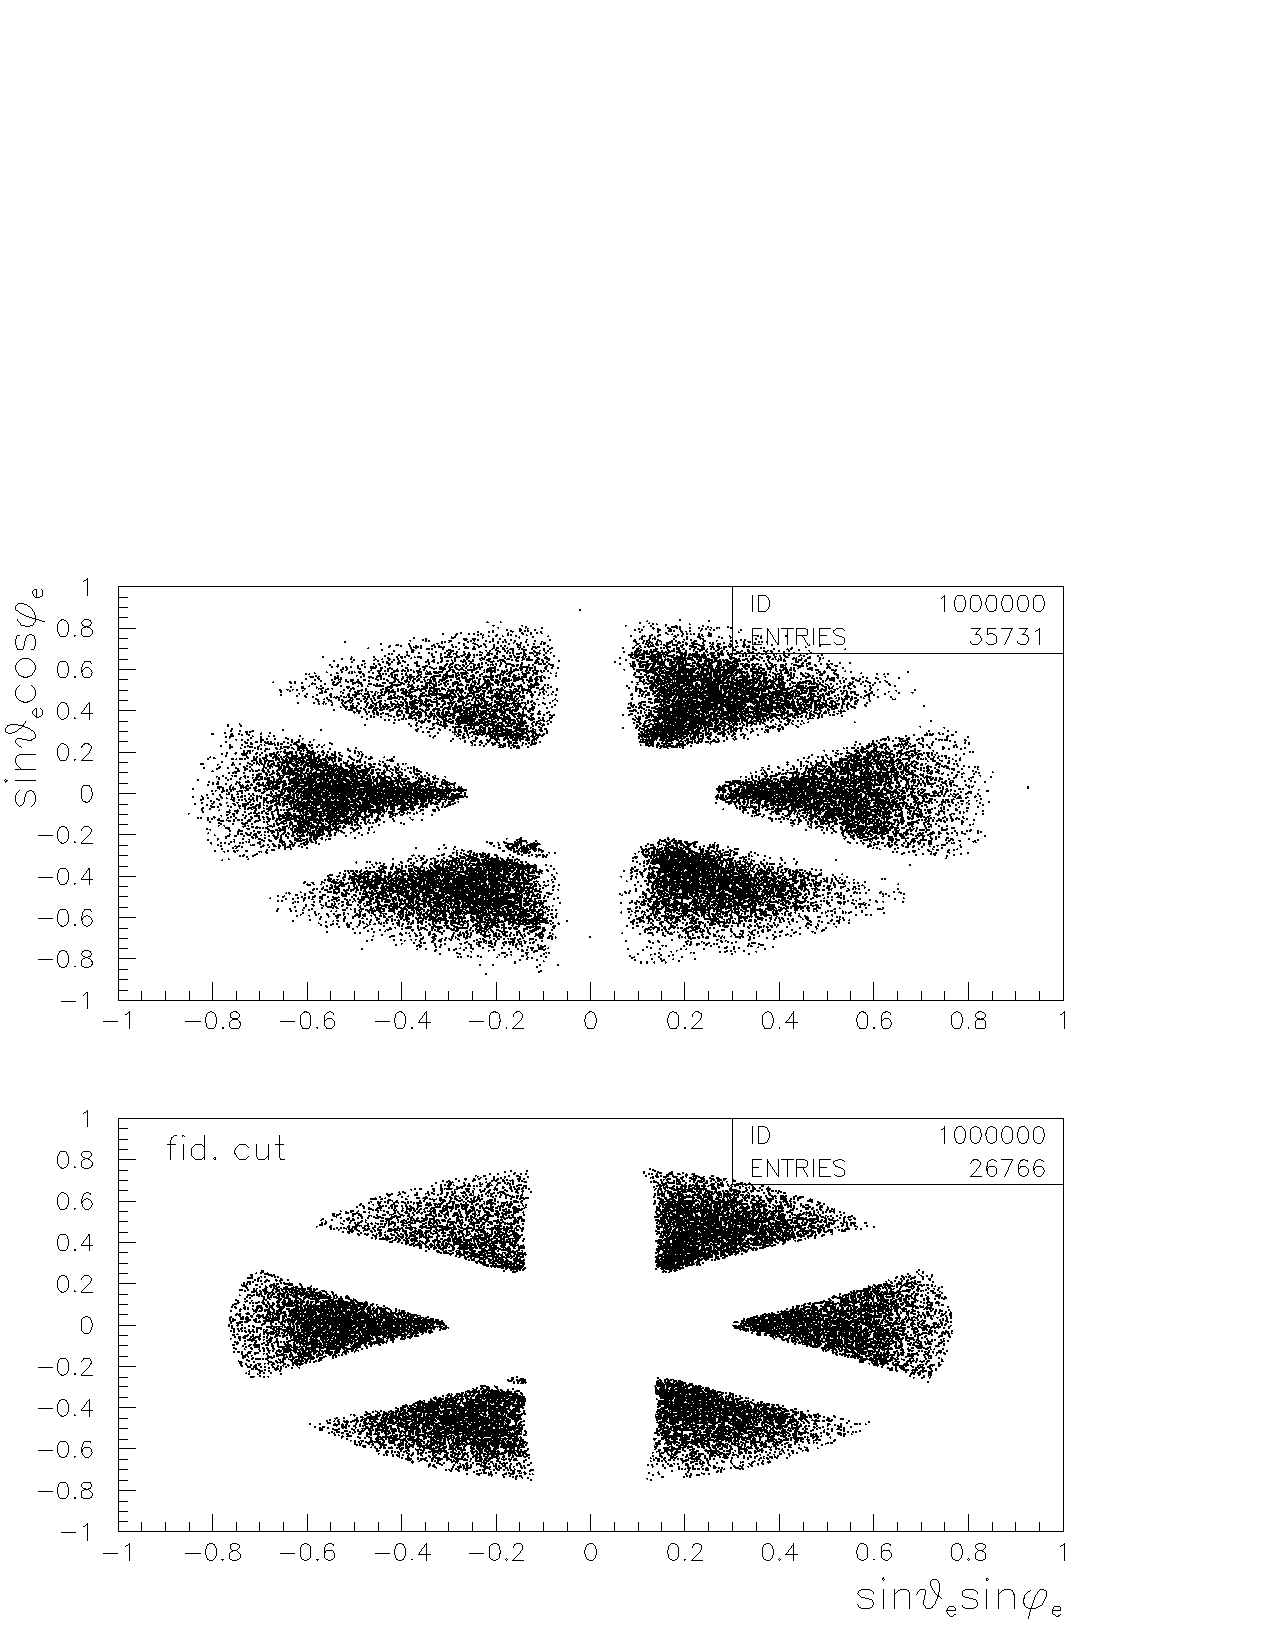
\includegraphics[width=0.8\textwidth]{plots/e16thvsphi.pdf}
   \caption{ Angular coverage of electrons without (top plot) and
with fiducial cut applied (bottom plot). }
 \label{fig:e16thvsphi}
 \end{figure} 

A vertex cut was applied to restrict the event sample to particles
with reconstructed vertexes in the target region 
(see Fig. \ref{fig:e16vertexcut}). The difference of electron and proton vertexes ($\Delta z = Z_e-Z_p$) was required to satisfy
$
-1.5 <\Delta z < -1.5 $ 
with  $-7.5+\Delta z < Z_e < *0.25 Z_e -2.0+\Delta z*0.25 $.


\begin{figure}
\centering
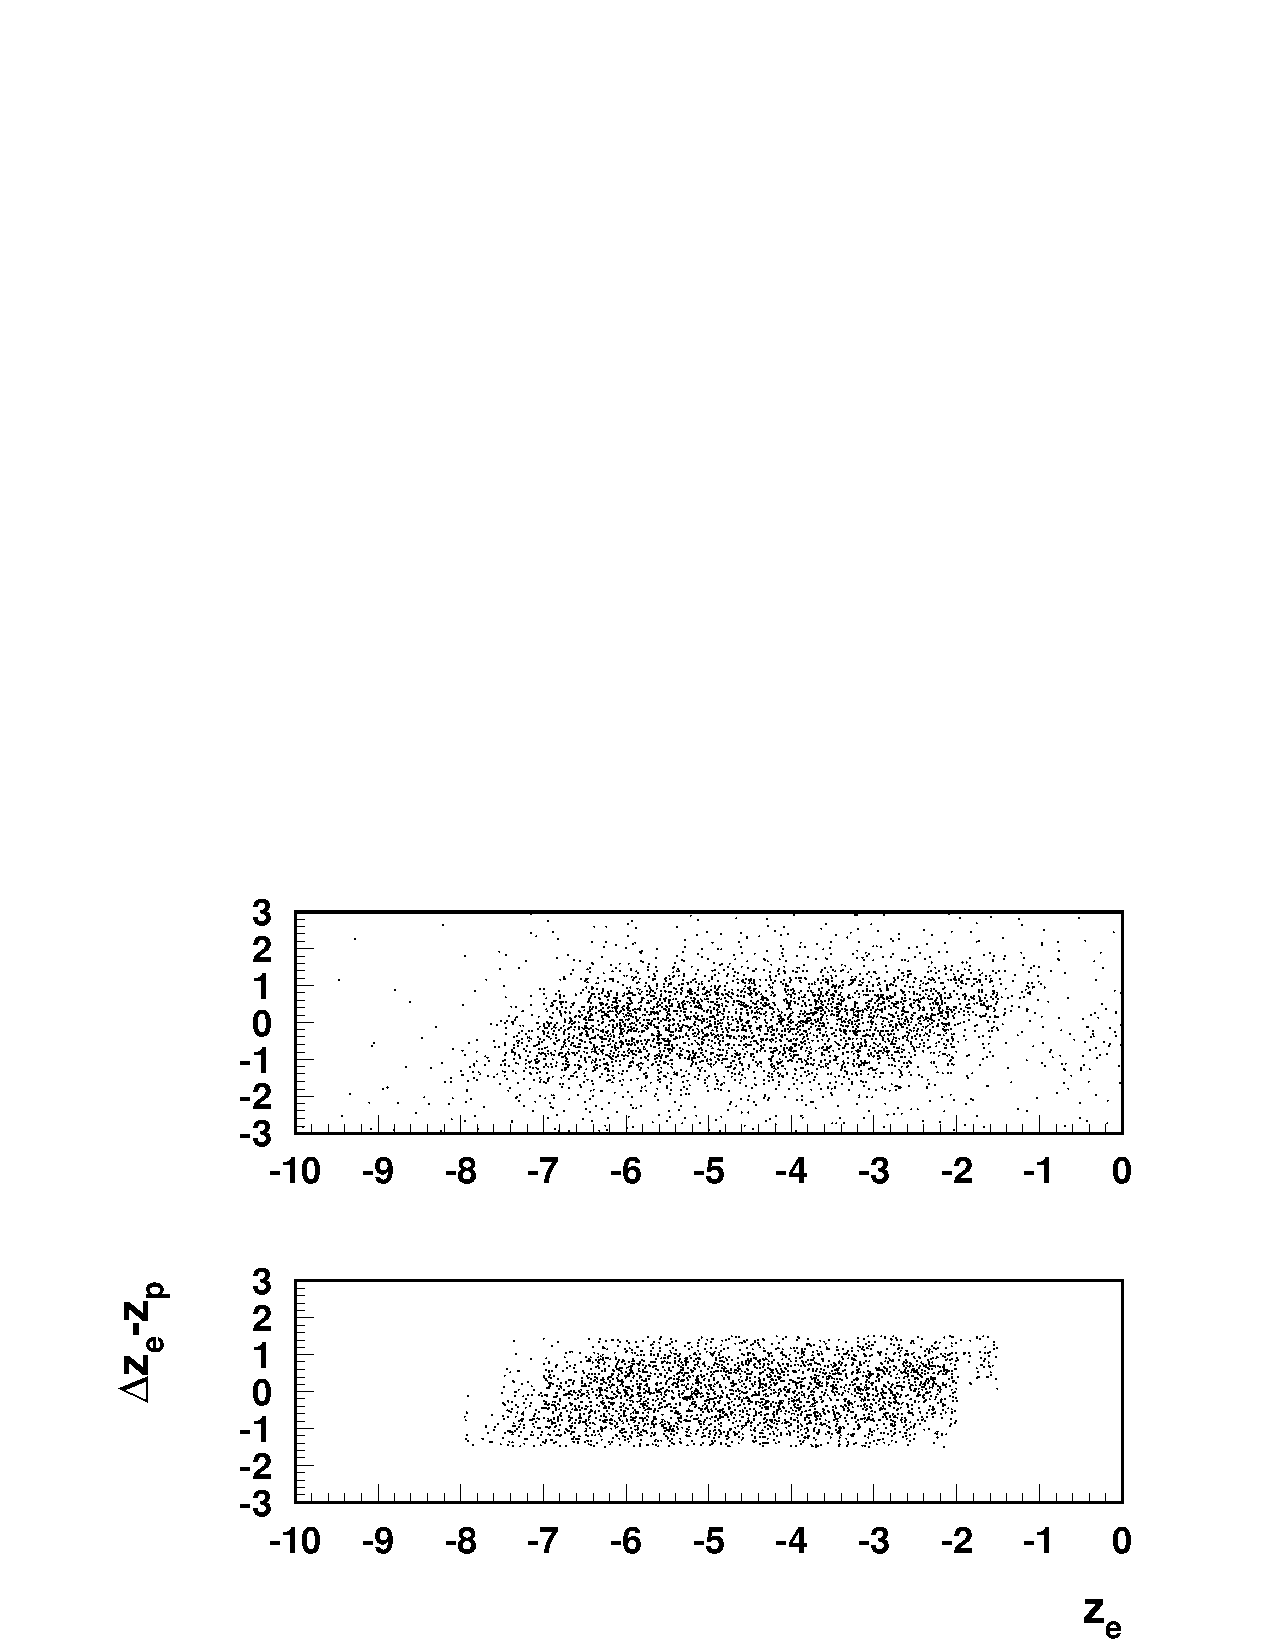
\includegraphics[width=0.8\textwidth]{plots/e16vertexcut.pdf}
   \caption{ Vertex cuts to data (bottom plot). }
 \label{fig:e16vertexcut}
 \end{figure} 

\subsection{Beam Polarization}

The average beam polarization, frequently measured  with a 
M{\o}ller polarimeter, was  $0.73 \pm 0.03$.

The  beam SSA  (see Fig. \ref{fig:dvcsalupass2nt21c}) was extracted on
run basis and used to check both the time stability of the SSA and
overall sign flips of the beam due to insertion of half wave plate.

\begin{figure*}[hptb]
\begin{minipage}{.6\textwidth}
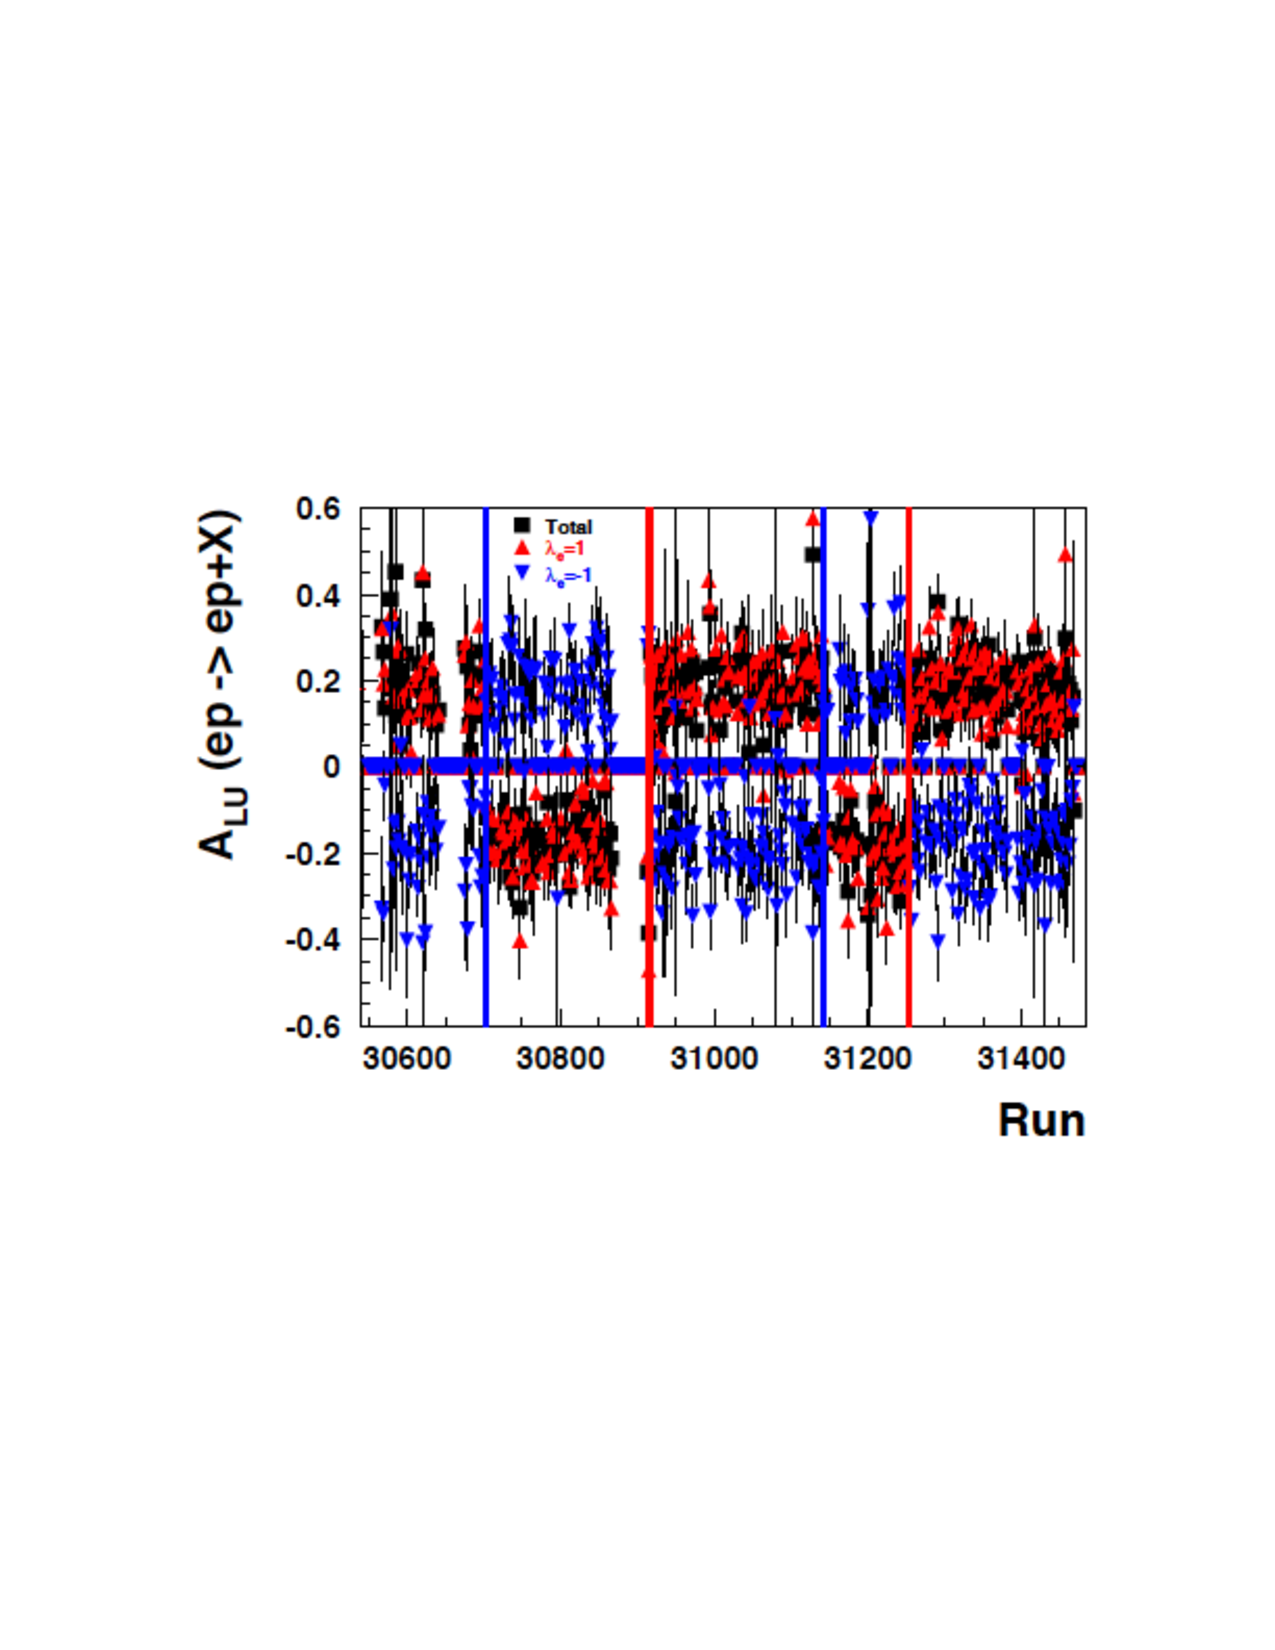
\includegraphics[width=9cm]{plots/dvcsalupass2nt21c.pdf}
\end{minipage}
\begin{minipage}{.6\textwidth}
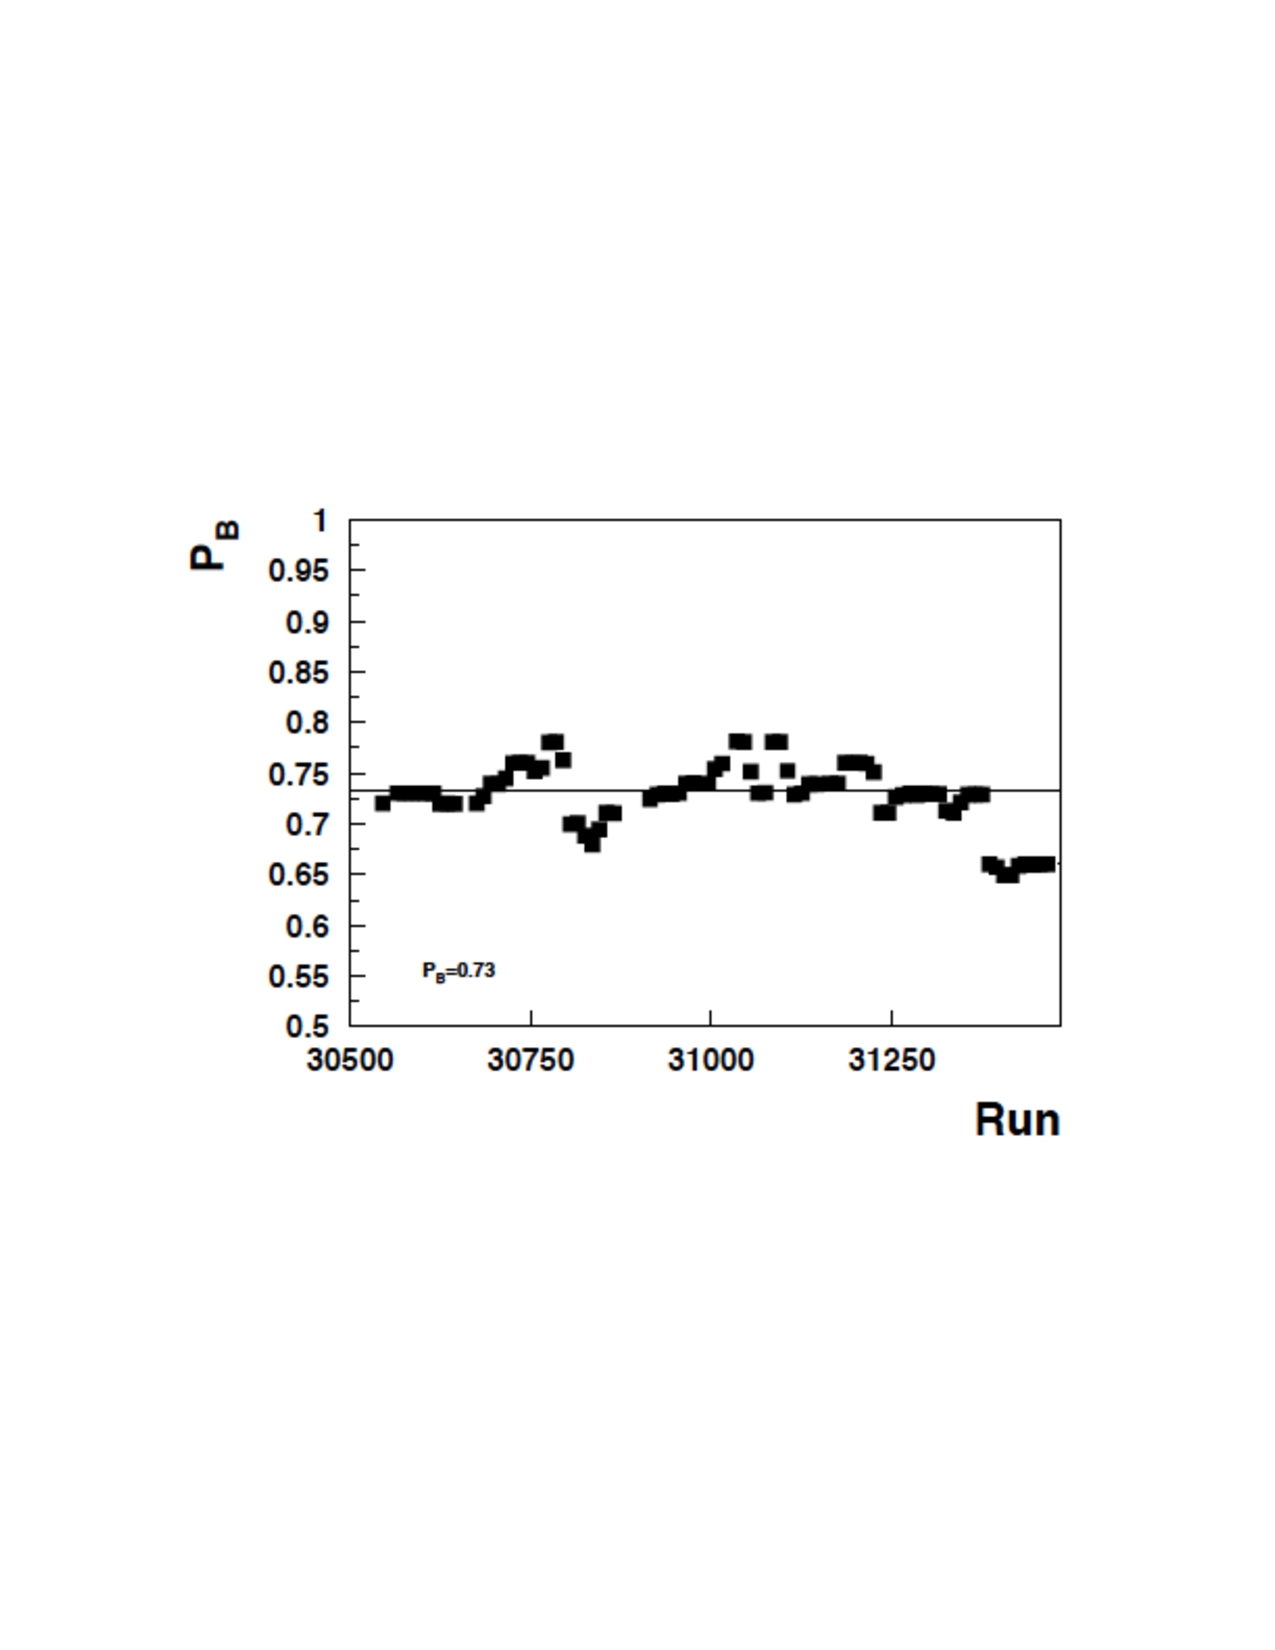
\includegraphics[width=9cm]{plots/e16beampol.pdf}
\end{minipage}
   \caption{ The raw beam-spin azimuthal asymmetry  dependence on the run number
for e16  run period (left) . Triangles up correspond to the positive helicity and triangles 
down to negative. Squares are for the difference. Beam polarization vs run number in e16 (right)}
 \label{fig:dvcsalupass2nt21c}
\end{figure*}


\begin{figure*}[hptb]
\begin{minipage}{.6\textwidth}
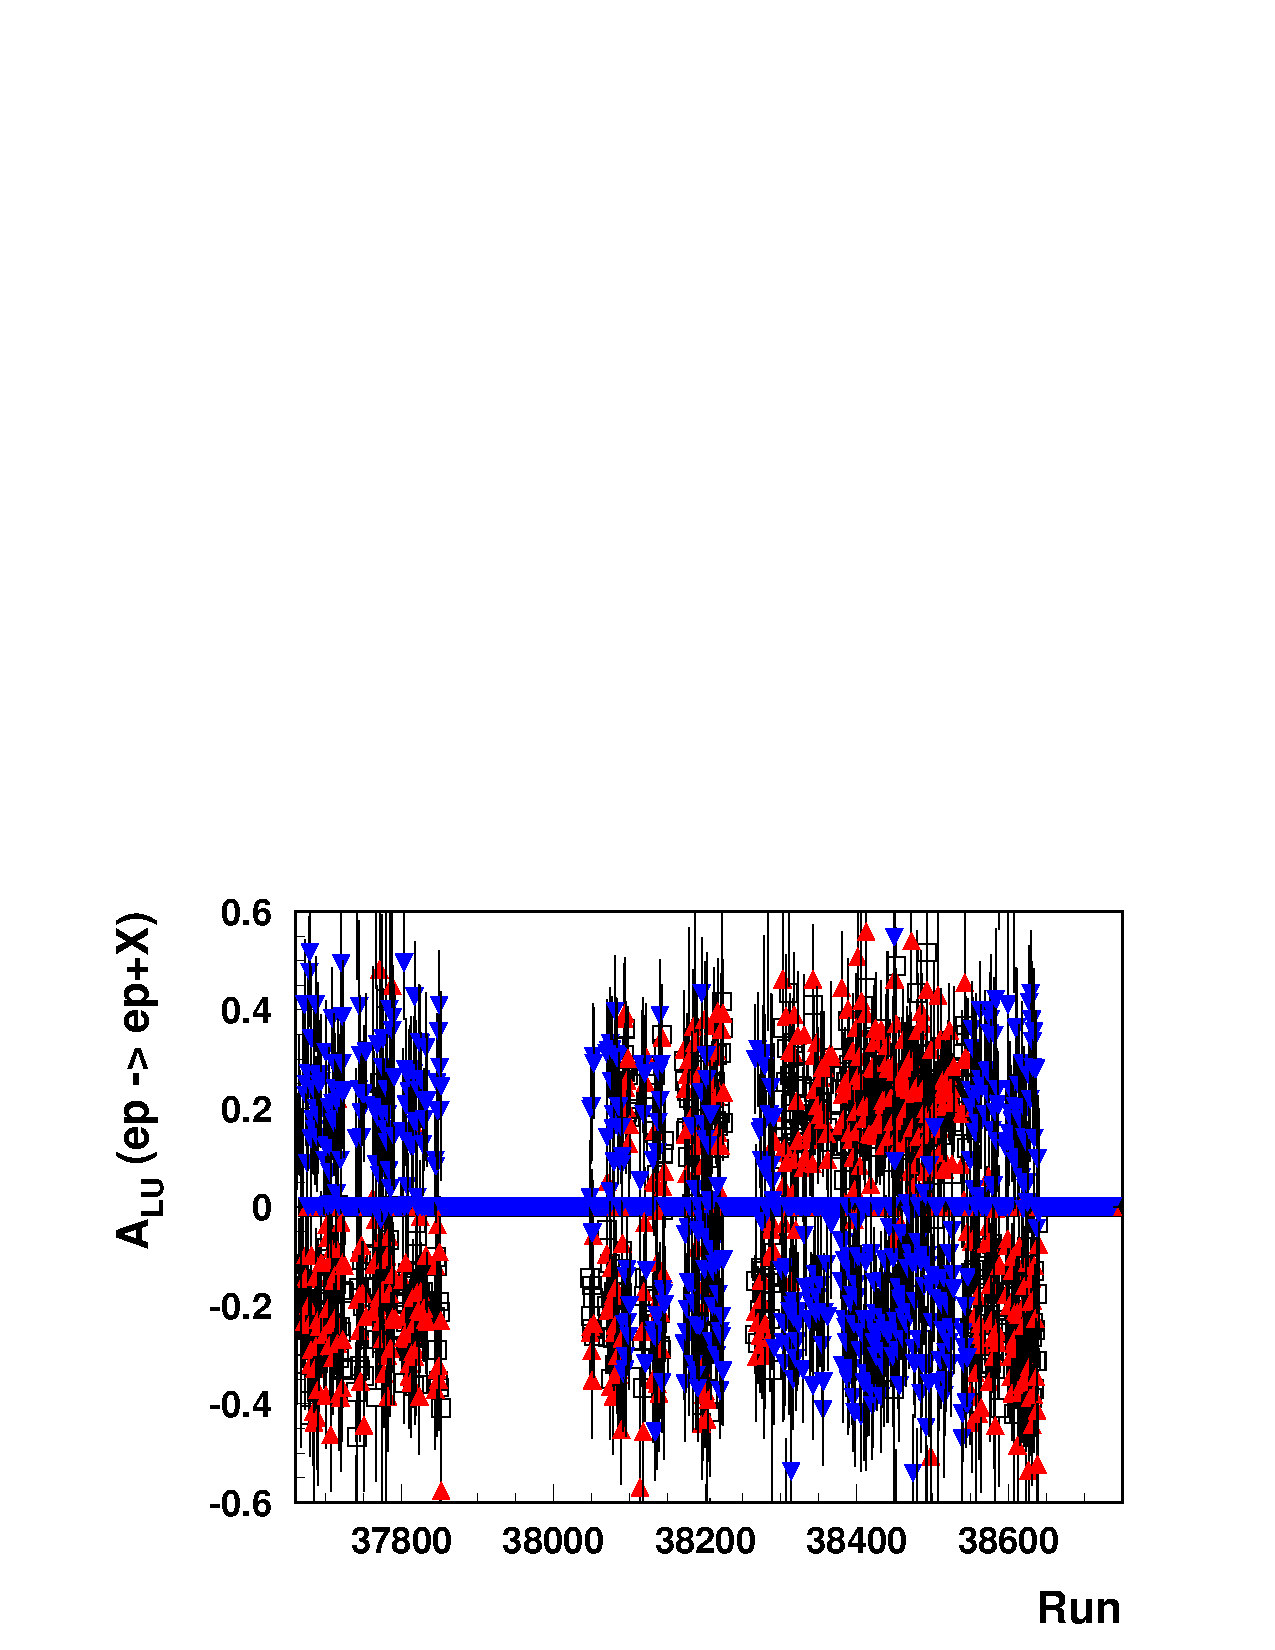
\includegraphics[width=9cm]{plots/dvcsalue1f-r37660-38750.pdf}
\end{minipage}
\begin{minipage}{.6\textwidth}
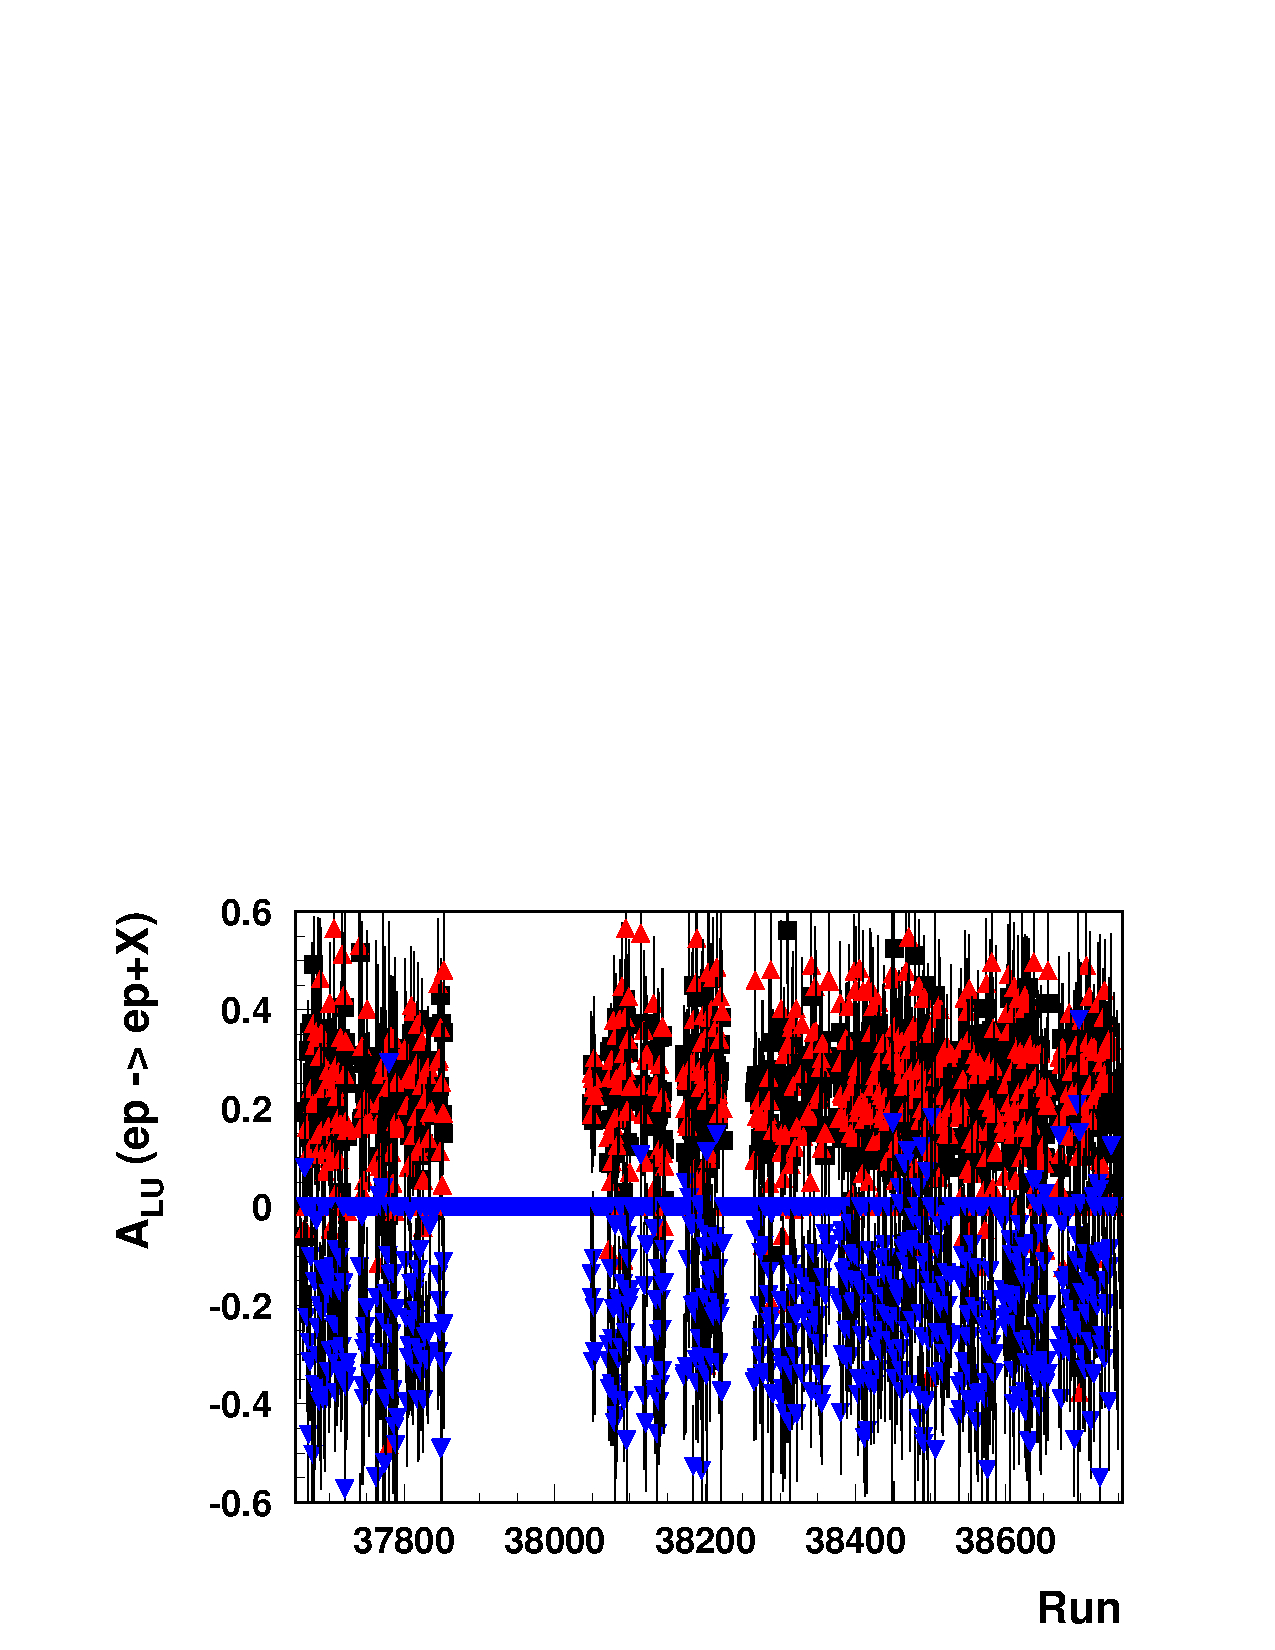
\includegraphics[width=9cm]{plots/dvcsalupass2nt21c-e1f.pdf}
\end{minipage}
   \caption{ The raw beam-spin azimuthal asymmetry  dependence on the run number
for e1f (right) run period. Helicity corrected asymmetry for e1f (right)}
 \label{fig:dvcsalupass2nt21c.e1f}
\end{figure*}



\subsection{Data selection and Particle Identification}
Additional to nt10 ids, cuts were applied on the calorimeter and Cerenkov to improve the
electron identification. 
The Fig. \ref{fig:e16recefficiency} shows reconstruction efficiency ratios for
data and MC, when applying fiducial cuts on CALO (2$\sigma$) and Cherenkov ($n_ph.e>2.5$),
compared to the basic sample with $e/p>0.12$ and $n_ph.e>0.5$.
As expected from the comparison between data and MC  the
most significant difference was observed at low $Q^2$, where the efficiency of the
Cherenkov counter is suppressing the low $Q^2$ (Fig. \ref{fig:e16recefficiency}).
Charged pions were primarily identified using the time-of-flight
scintillators. The upper plots in 
Fig.~\ref{pidpi} shows the time difference (TOF)
between the observed and expected arrival time for a charged pion of 
a given momentum, using the trigger electron to define the
start time at the target. Only plotted are events satisfying the electron
cuts mentioned above, the additional kinematic cuts
$0.4<z<0.7$ and  $M_X>1.4$ GeV used in the principal semi-inclusive
analysis. Cut on the fraction of the virtual photon energy
carried by the pion, $z$, is based on the previous SIDIS studies performed at Hall-C, CLAS and HERMES and is supposed
to restrict the kinematics to the region where contributions from the target fragmentation and exclusive processes 
are not significant.  
In the case of positive particles (upper left plot),
a large slanted side-band is seen in the upper left of the plot,
corresponding to protons.  Above $P=1.6$ GeV, the pion/kaon contamination
grows to an estimated level of  about 5\%. In the present analysis,
a detailed bin-by-bin subtraction of kaon/pion contamination was not
done (it may well depend not only on $P$, but also on $M_x$, $W$,
$Q^2$, and $P_T$), as justified by the preliminary nature of the present
study. It should be done, however, for the much higher statistical
accuracy expected from upcoming experiments, for which the present
study can be considered as a pilot investigation.

\begin{figure*}[hptb]
\centering
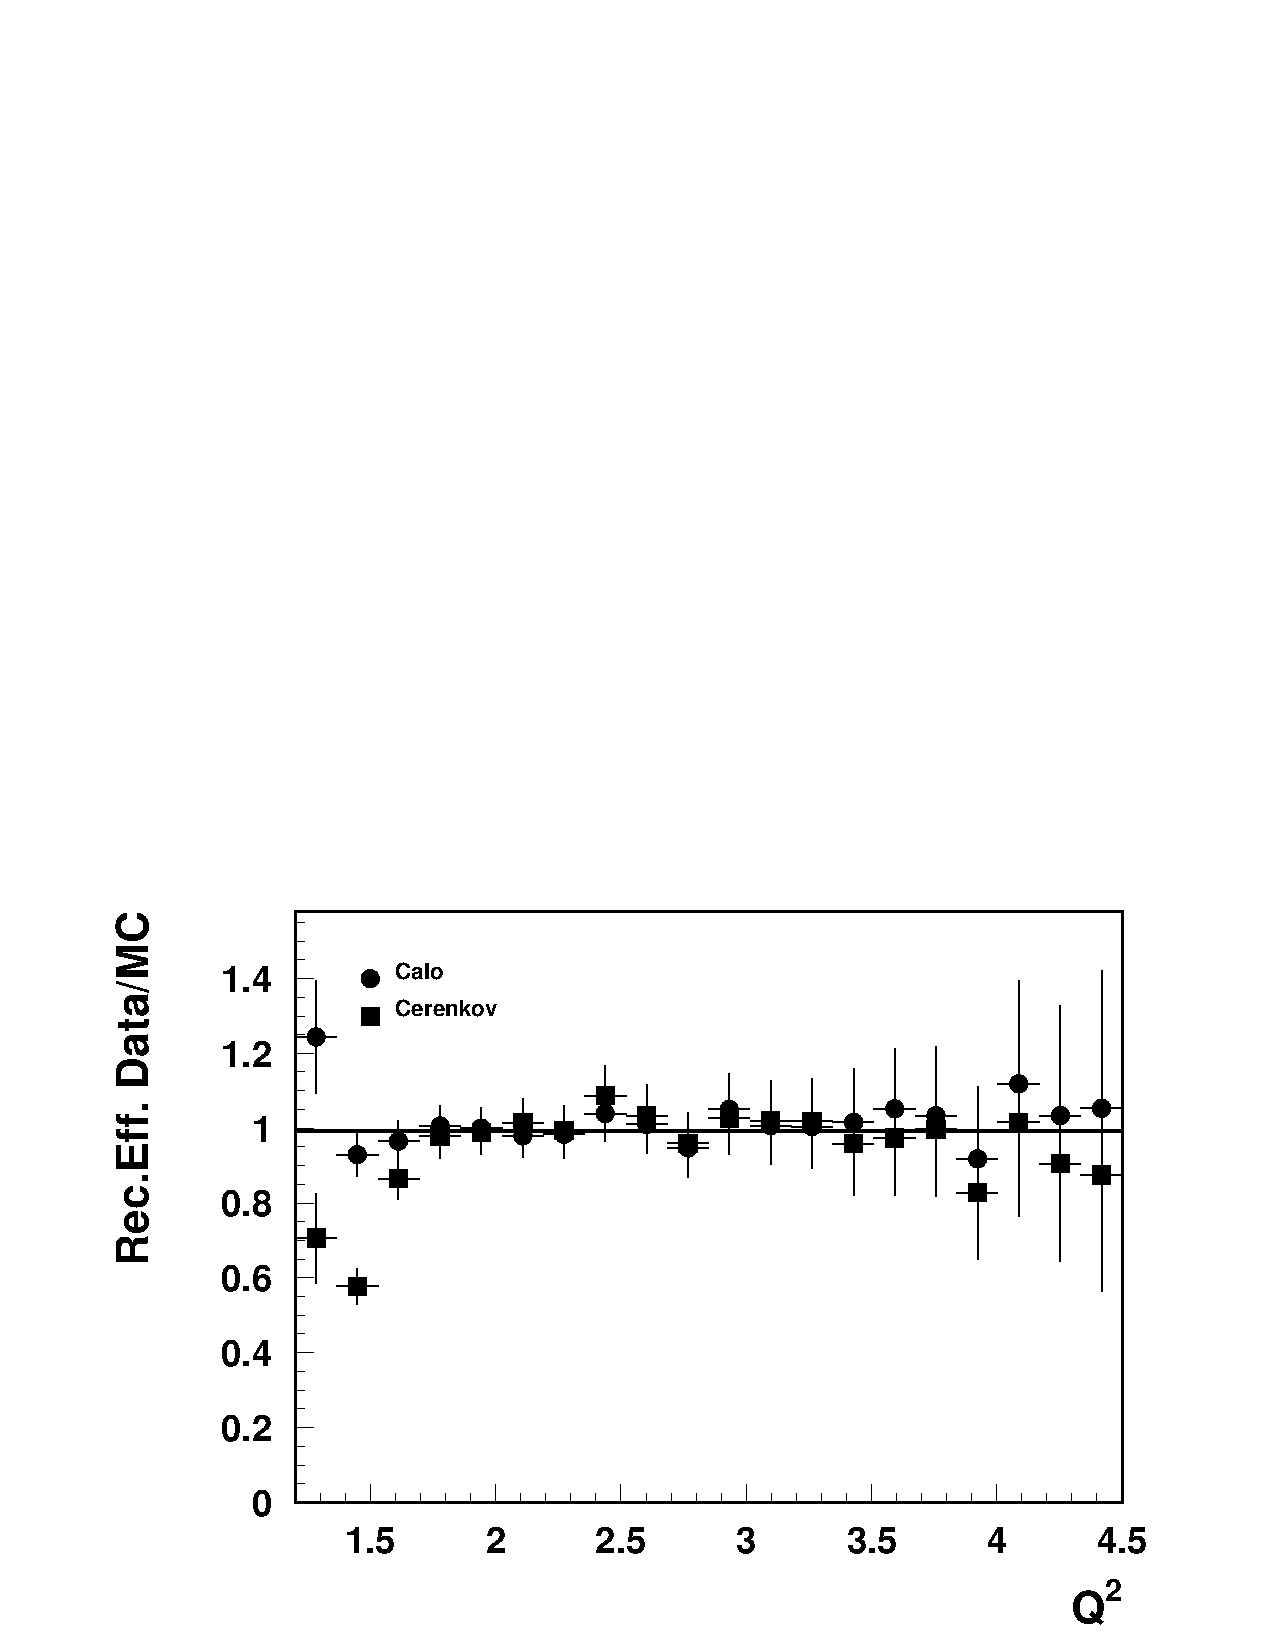
\includegraphics[width=0.6\textwidth]{plots/e16recefficiency.pdf}
   \caption{Reconstruction efficiency of CALO and Cherenkov as a function of  $Q^2$.}
 \label{fig:e16recefficiency}
\end{figure*}

\begin{figure}[hbt]
\includegraphics[width=0.6\textwidth]{plots/piontof.pdf}
\caption{Upper: Time-of-flight difference from that expected
for electron-pion coincidences as a function of momentum
for positive (negative) hadrons on left (right). The red lines
indicate the cuts used. Lower: Cherenkov counter signals 
for hadron candidates for positive (negative) hadrons on left (right) }
\label{pidpi}
\end{figure}

\subsection{Momentum Corrections}

Major corrections affecting the missing mass distributions of $ep$ sample
include the proton energy loss corrections and electron momentum corrections.
 

\subsubsection{Momentum corrections}
The momentum corrections were performed using as input the exclusive sample
of  $ep\pi^+\pi^-$ events extracted from e16 data set (after applying energy
loss corrections based on the MC) to the momcor program developed by S.Kuhn \cite{Kuhn:e6}.
The effect of the energy loss corrections on the missing energy for the 
$ep\pi^+\pi^-$ sample is shown on Fig. \ref{fig:e16energybalance}.
\begin{figure}
\begin{minipage}{.6\textwidth}
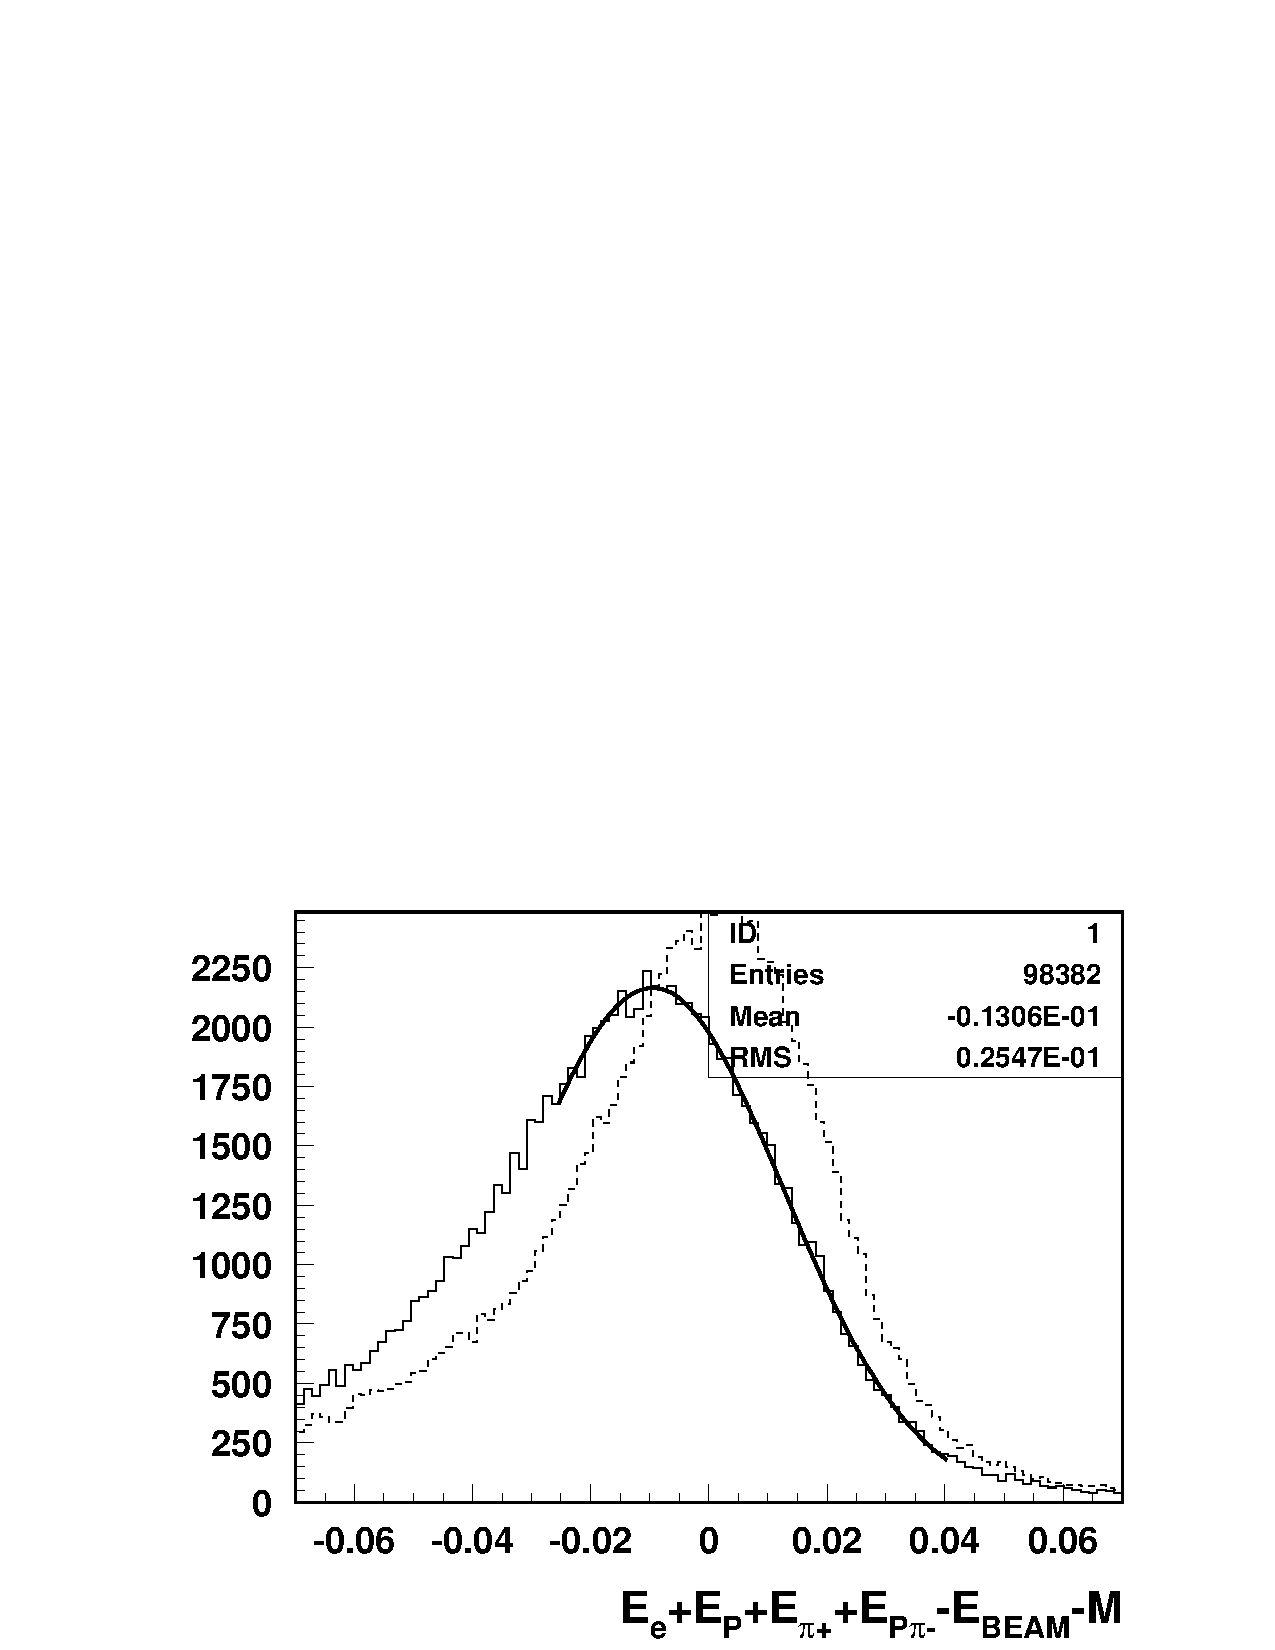
\includegraphics[width=9cm]{plots/e16energybalance.pdf}
\end{minipage}
\begin{minipage}{.6\textwidth}
\includegraphics[width=9cm]{plots/e16momcor.pdf}
\end{minipage}
   \caption{Missing energy of the exclusive $ep\pi^+\pi^-$
     sample  with solid/dashed lines showing it before and after corrections using the momcor \cite{Kuhn:e6} (left). The energy balance of exclusive $ep\pi^+\pi^-$
sample from e16 before (solid line) and after (dashed) energy loss corrections (right).}
 \label{fig:e16energybalance}
 \end{figure} 
The missing mass of  $e\pi^+\pi^-X$ before and and after
momentum corrections is shown in Fig. \ref{fig:e16energybalance} (right panel). 

\section{SSA in b2b hadron production}


A study using unpolarized SIDIS in Hall C at Jefferson Lab
concluded that significant deviations from the leading order
factorized model (SIDIS described as the product of quark
distributions and fragmentation functions) only occur for $M_X<1.4$
GeV~\cite{Navasardyan:2006gv}. 

The $P_T$-dependence is illustrated in Fig.~\ref{fig:b2bpt}. The
data show a trend for asymmetry to increase with increasing transverse momenta of pion and proton $P_{T1}$,$P_{T2}$,
consistent with expectations from theory. 
The final asymmetry, after kinematic corrections due to different $\xbj$-averages 

The $z$-dependence is illustrated in Fig.~\ref{fig:b2bz}. 
The contamination from target
fragmentation, higher twist, or other effects are important
for $z<0.3$. This seems reasonable, because only for $z>0.5$ can 
one be sure that a pion is ``leading'' (i.e. the highest
momentum pion in the fragmentation process, hence the one
most closely associated with the struck quark).
Based on previous studies we have chosen $0.7>z>0.4$ as the canonical cut. With $M_X>1.4$ cut we have almost
no data at $z>0.7$, but we use this cut as it was determined in Hall C that
strong deviations for the quark-parton model occur at 
high $z$~\cite{Navasardyan:2006gv}.
%
We first examine the $x$-dependence, as illustrated in Fig.~\ref{fig:Allx}.
The  $A_{LU}$
increases with $x$ due to the increasing dominance of polarized $u$ quarks,
which have positive polarization.

\begin{figure}
\begin{minipage}{.6\textwidth}
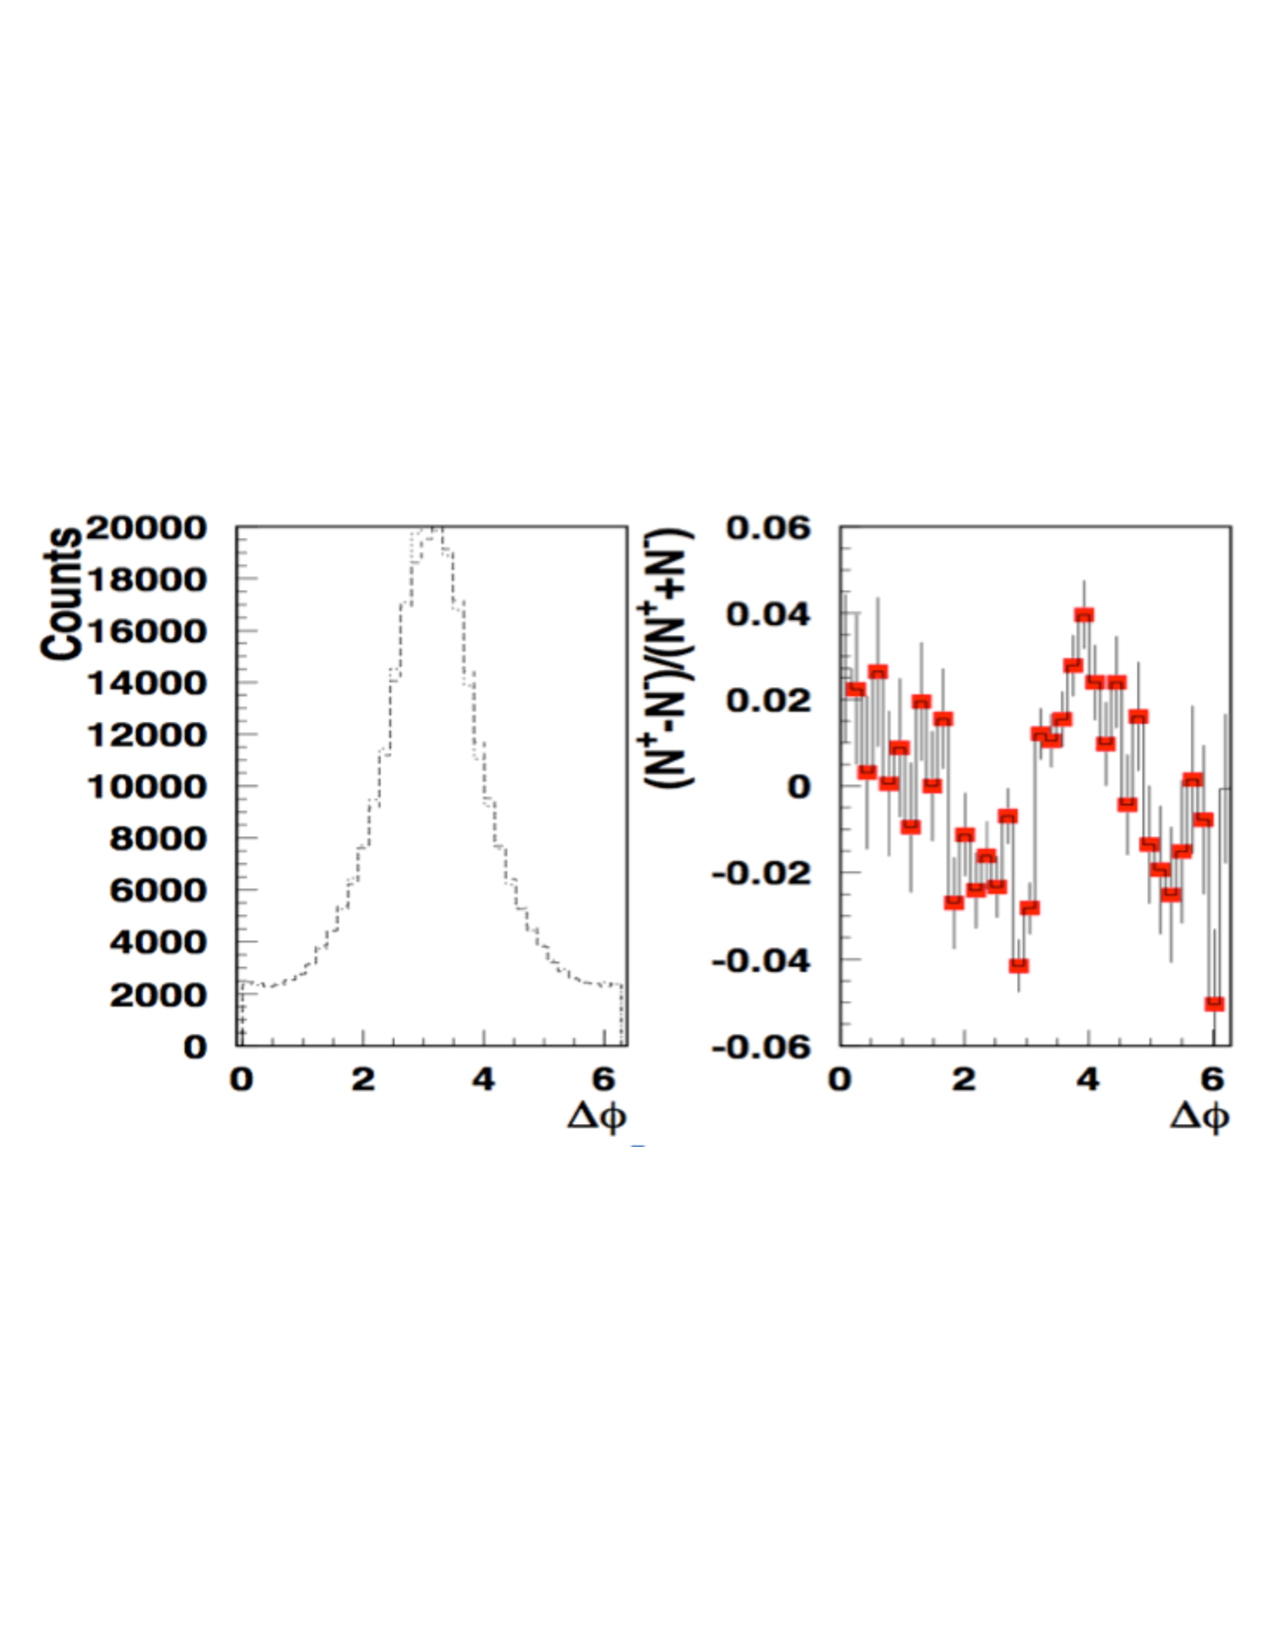
\includegraphics[width=9cm]{plots/b2b-sinus.pdf}
\end{minipage}
\begin{minipage}{.6\textwidth}
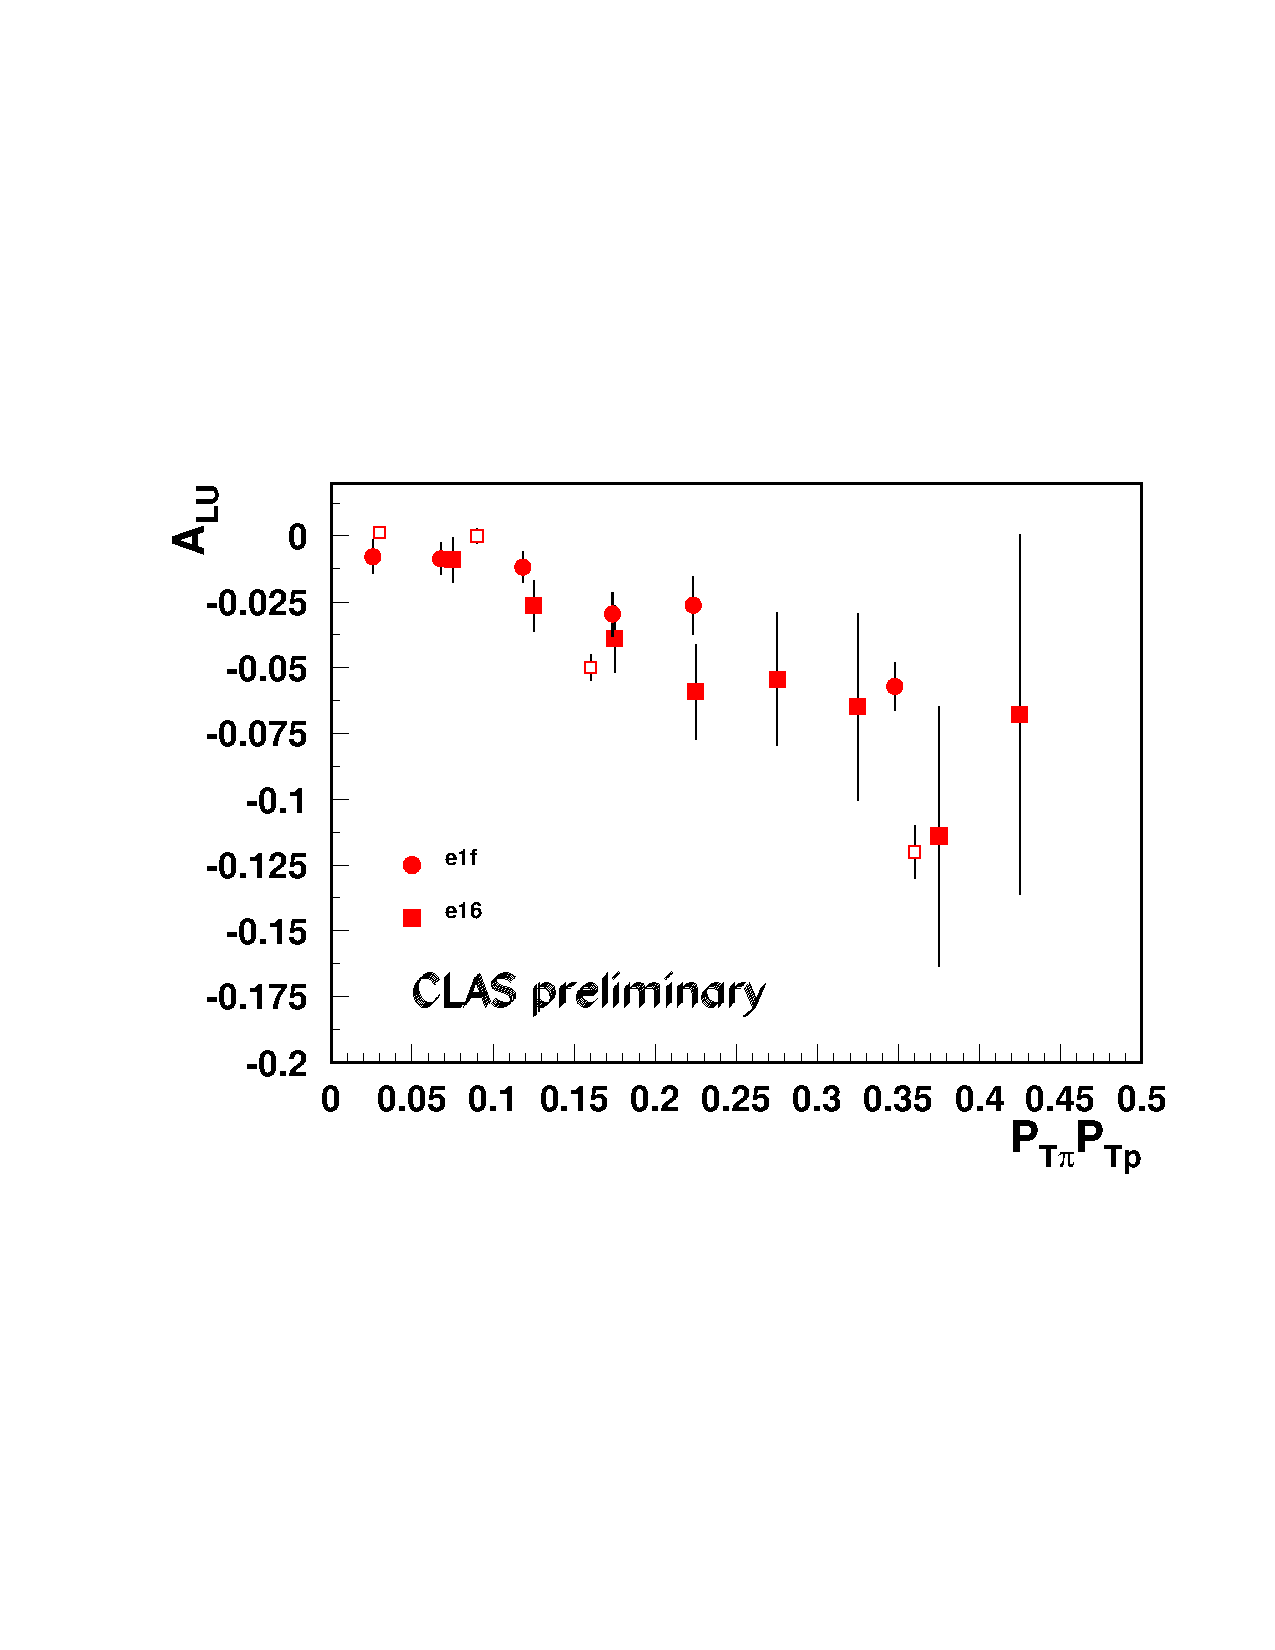
\includegraphics[width=9cm]{plots/dr-b2b-pip-pt-bin36-z04-07-x01-06-pt0-065-min2.pdf}
\end{minipage}
   \caption{Lepton single-spin asymmetry in $ep\rightarrow e^\prime p\pi^+$ as a function of the $\Delta \phi$ (left). 
$A_{LU}$ dependence on product of transverse momenta of final state proton and $\pi^+$ (right).}
 \label{fig:b2bpt}
 \end{figure} 

\begin{figure}
\begin{minipage}{.6\textwidth}
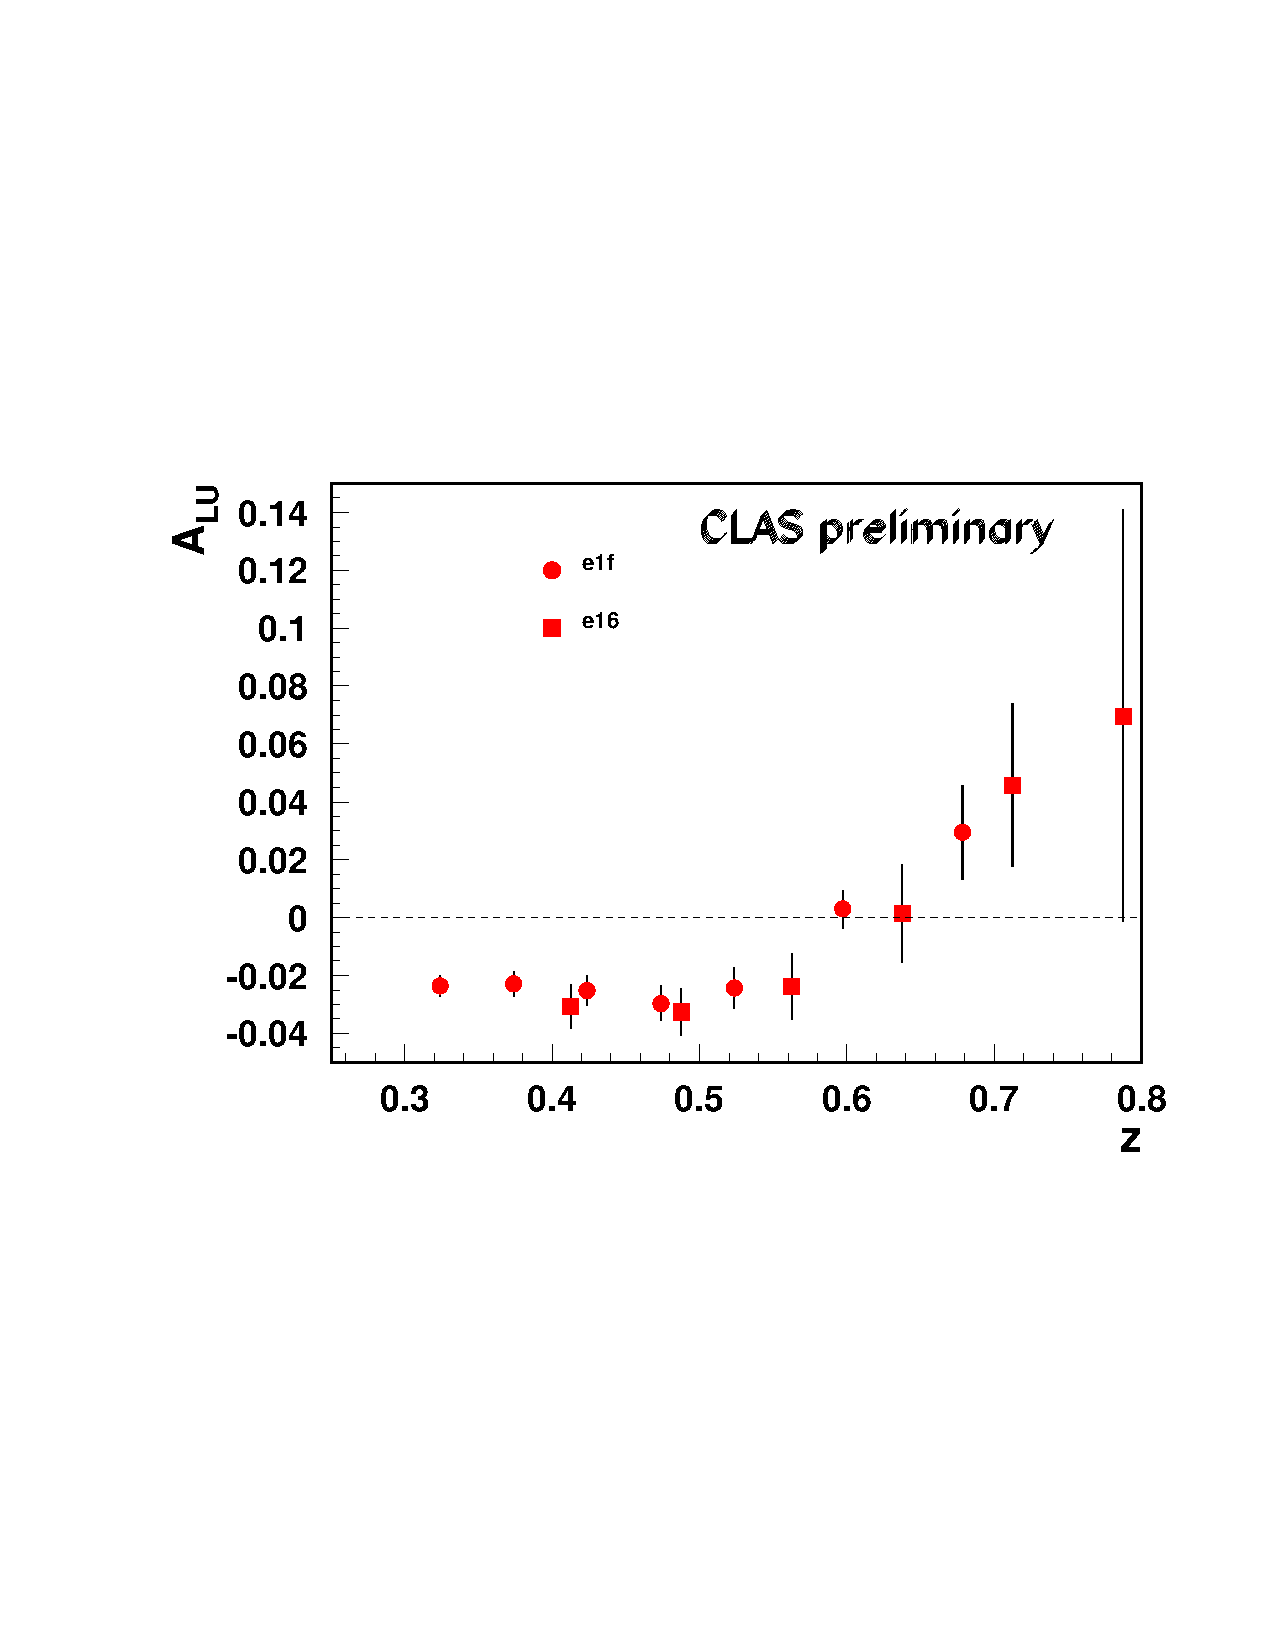
\includegraphics[width=9cm]{plots/dr-b2b-pip-z-bin36-z04-07-x01-06-pt0-065-min2.pdf}
\end{minipage}
\begin{minipage}{.6\textwidth}
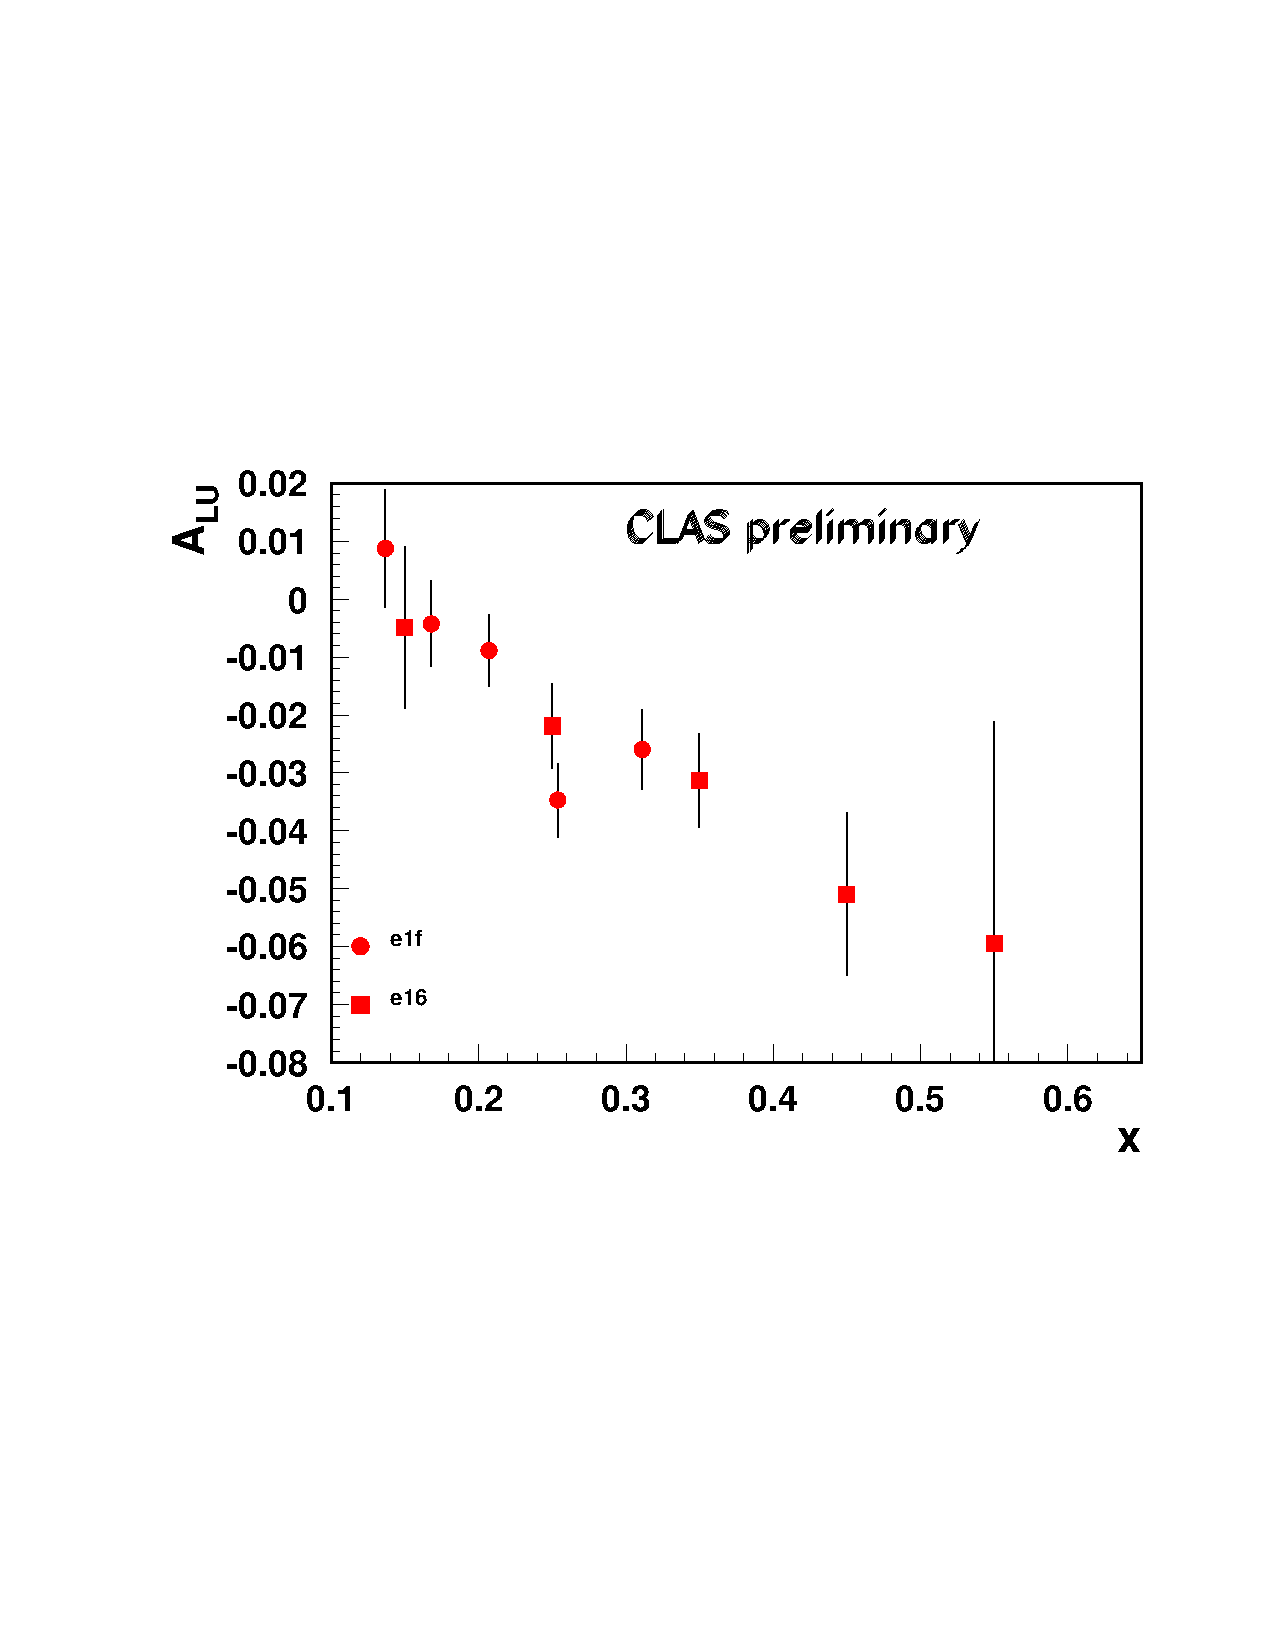
\includegraphics[width=9cm]{plots/dr-b2b-pip-xf-bin36-noexc-acc-xm-aluvsmmas-new-dsin2-z04-07-x01-06-pt0-065-min2.pdf}
\end{minipage}
   \caption{$A_{LU}$ z-dependence, integrated over other kinematical variables(left). 
$A_{LU}$ dependence on $\xbj$ for $0.4<z<0.7$ $\pi^+$ (right).}
 \label{fig:b2bpt}
 \end{figure} 

Similar behaviour has been observed also for events with neutral and negative pions in the final state, detected in coincidence with
scattered electron and proton in the target fragmentation region.
The dependence of the $A_{LU}$ for $ep\pi^-$ and  $ep\pi^0$  is shown in
in Fig. \ref{fig:b2b-pionpt}

\begin{figure}
\begin{minipage}{.5\textwidth}
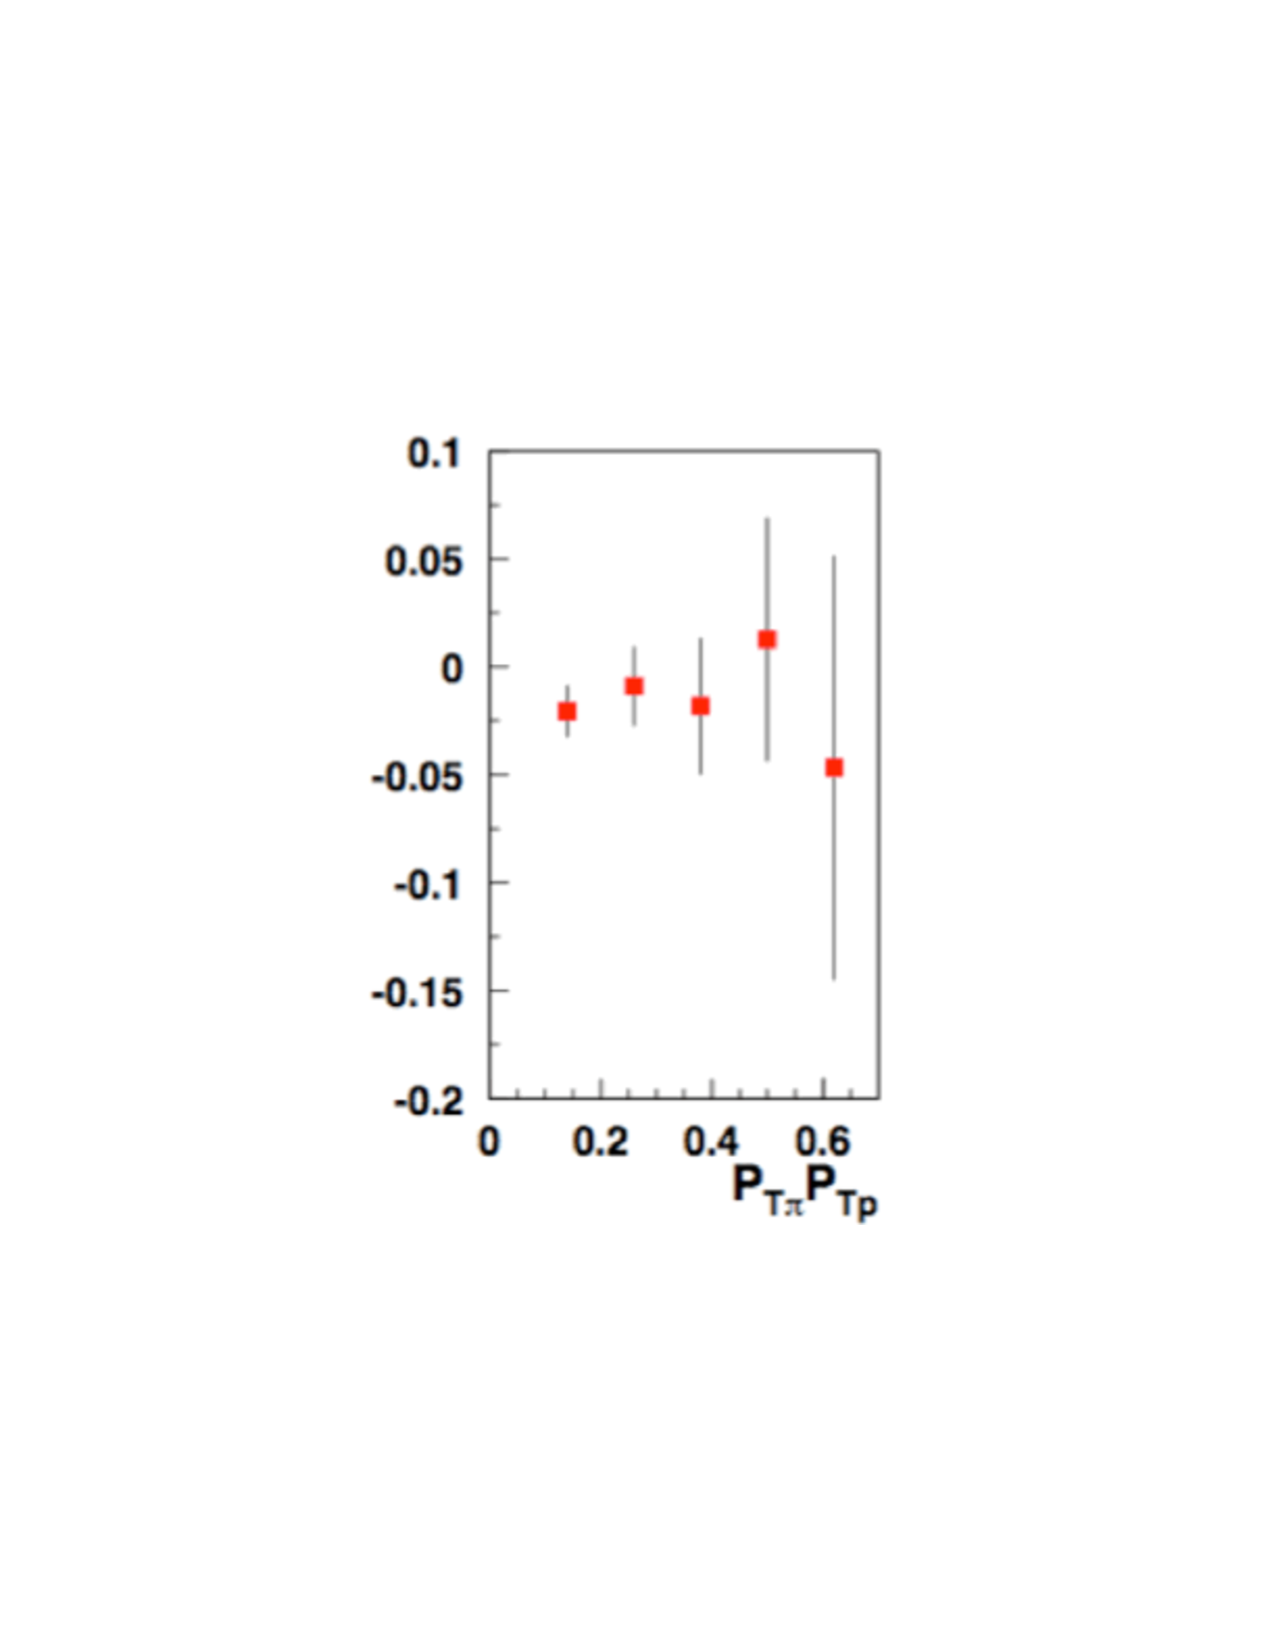
\includegraphics[width=8cm]{plots/b2b-pimpt.pdf}
\end{minipage}
\begin{minipage}{.5\textwidth}
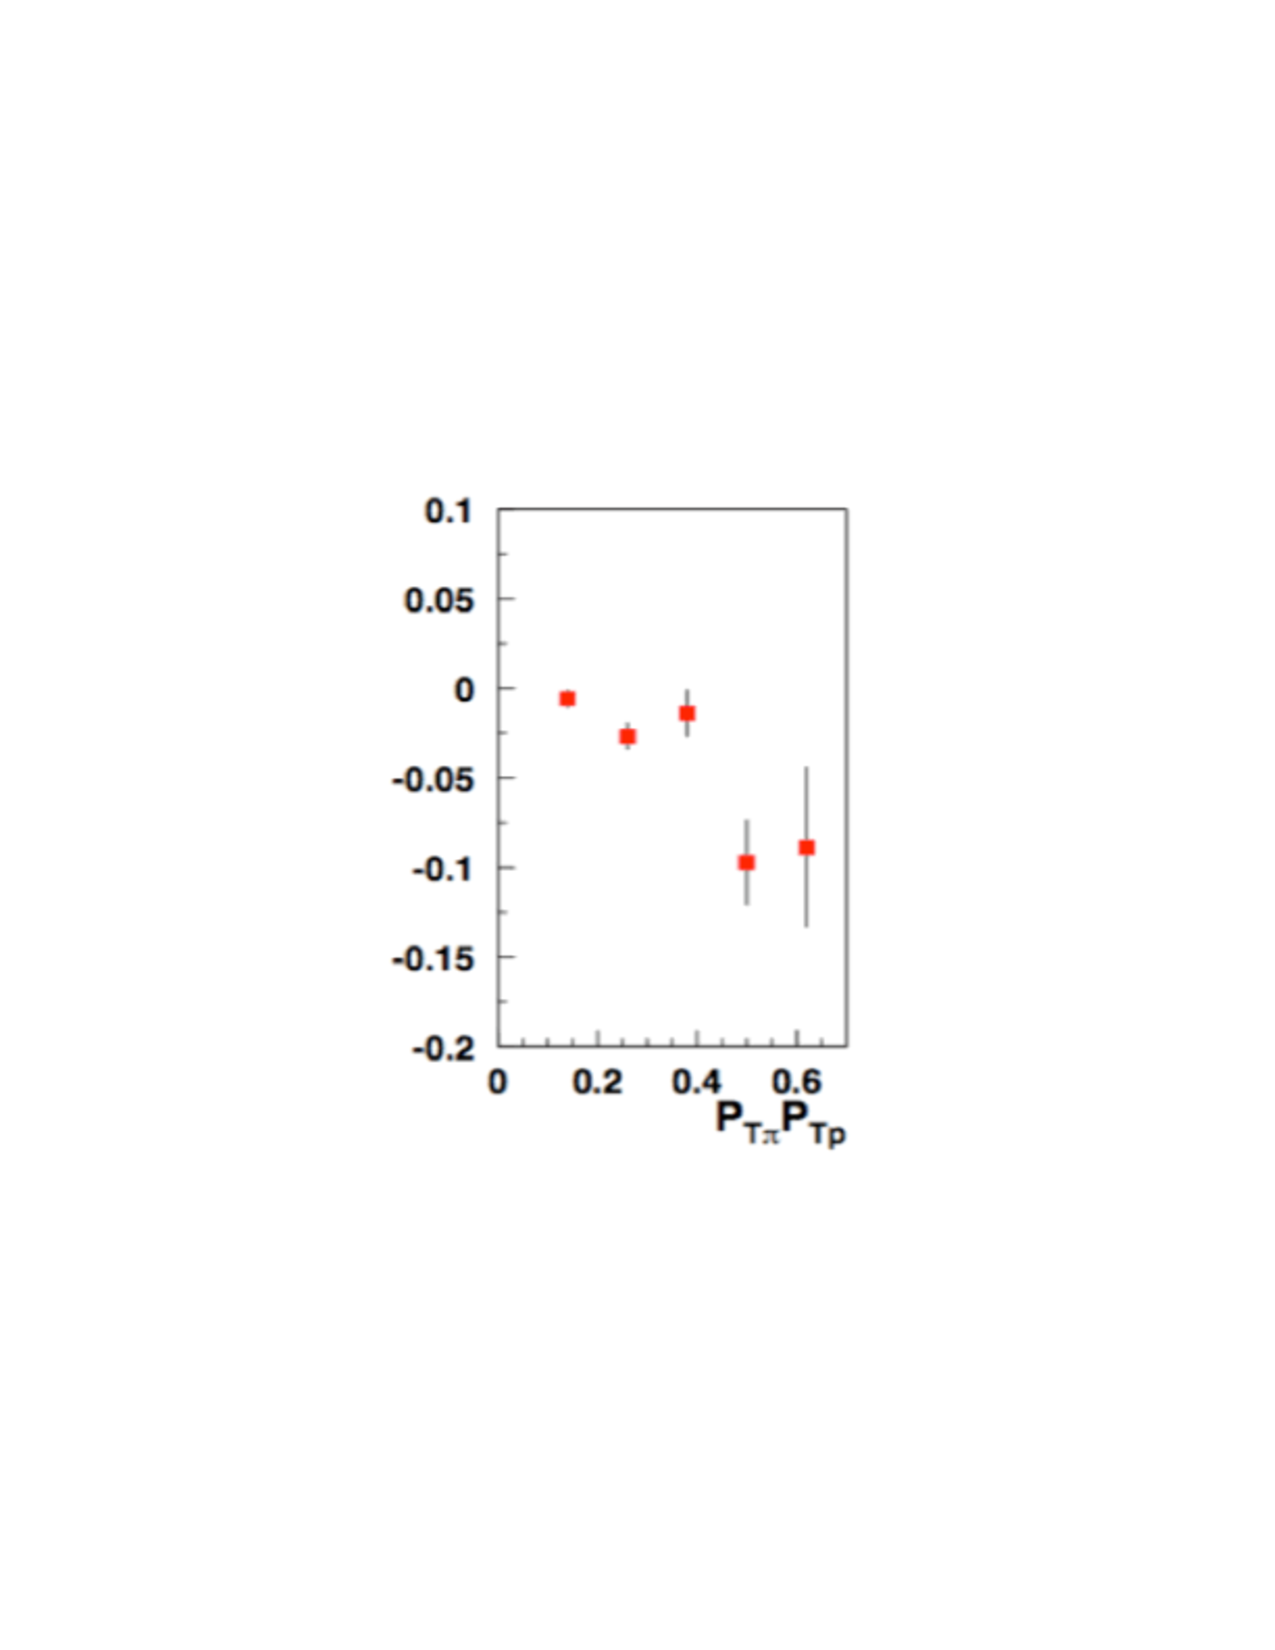
\includegraphics[width=9cm]{plots/b2b-pi0pt.pdf}
\end{minipage}
   \caption{$A_{LU}$ dependence on $P_{T\pi}P_{Tp}$ for the  $ep\pi^-$  (left) and  $ep\pi^0$ (right) events.}
 \label{fig:b2b-pionpt}
 \end{figure} 


The missing mass dependence of the $A_{LU}$ for all three pions is shown
in Fig. \ref{fig:b2b-mx3}
\begin{figure}
\hskip -2cm
\begin{minipage}{.35\textwidth}
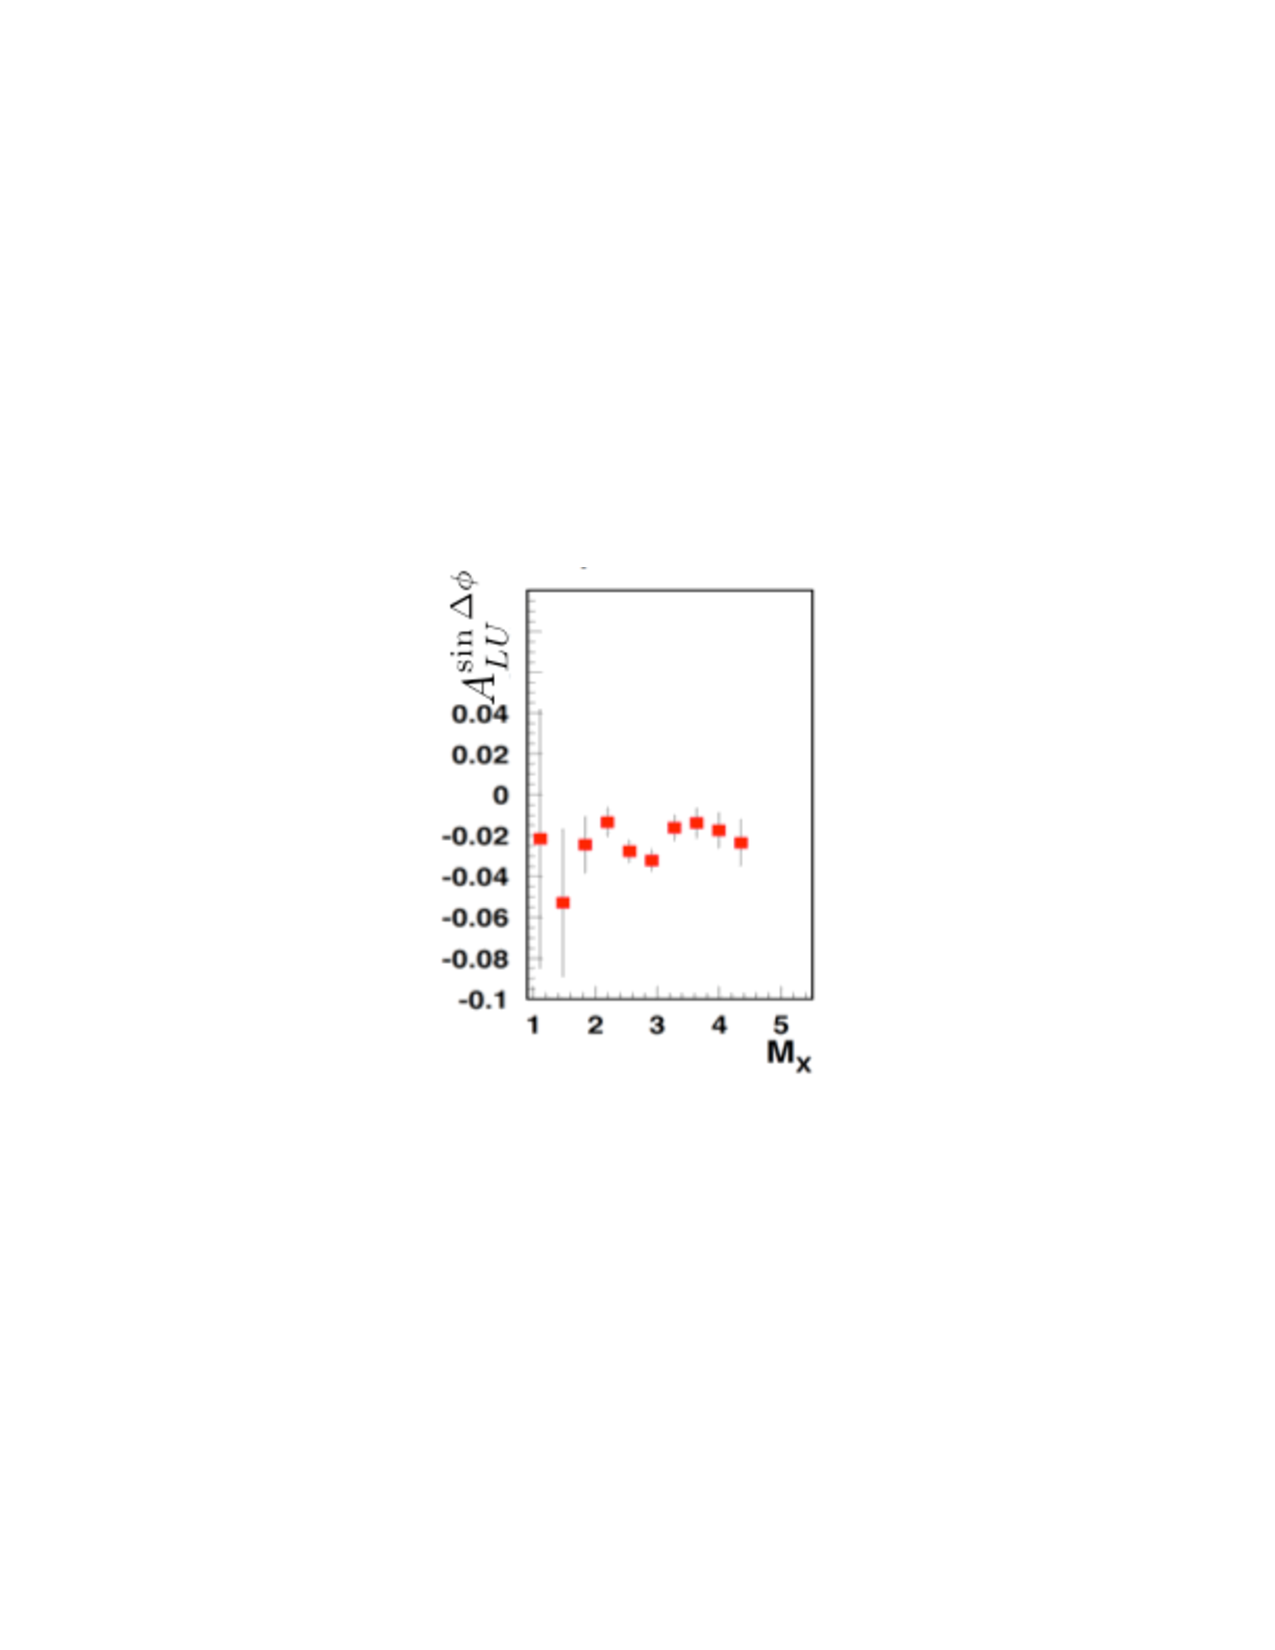
\includegraphics[width=10.0cm,height=10cm]{plots/alu-pipmx.pdf}
\end{minipage}
\begin{minipage}{.2\textwidth}
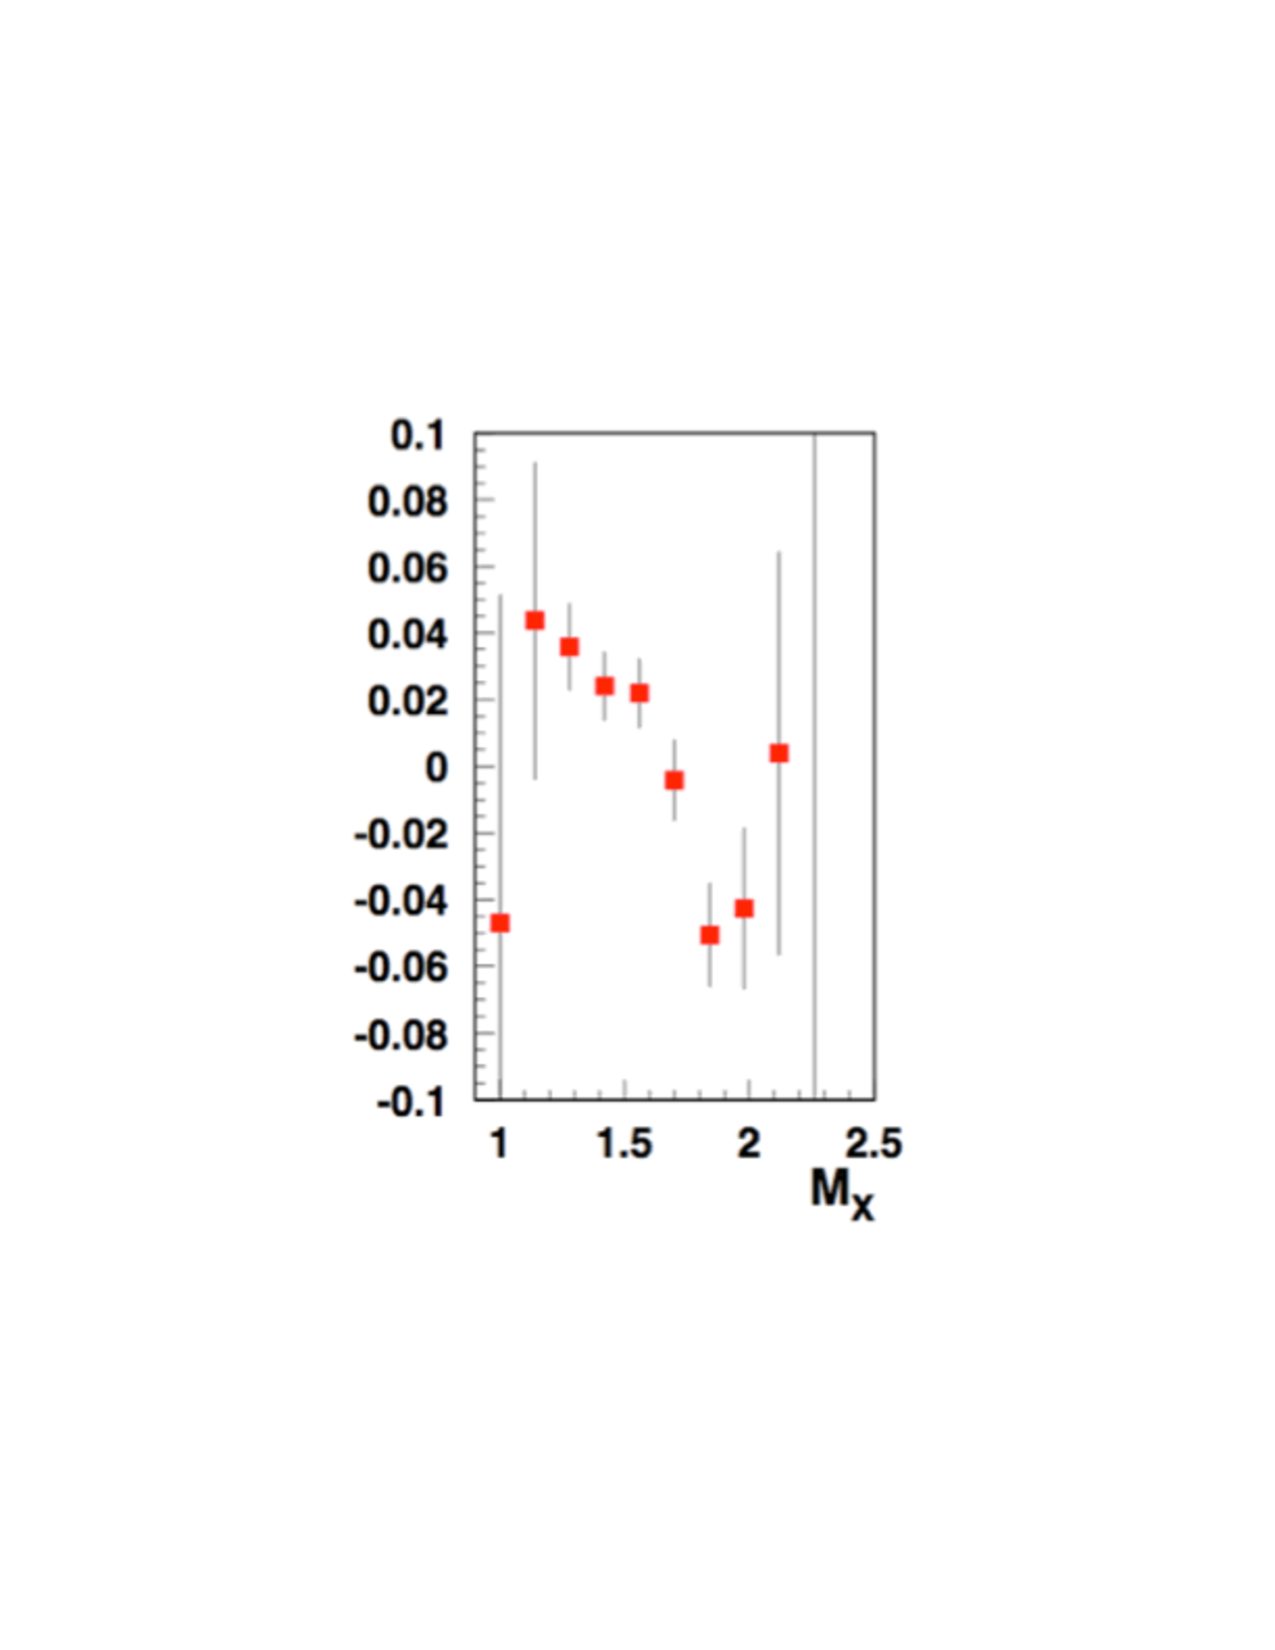
\includegraphics[width=7.2cm,height=6cm]{plots/alu-pimmx.pdf}
\end{minipage}
\begin{minipage}{.3\textwidth}
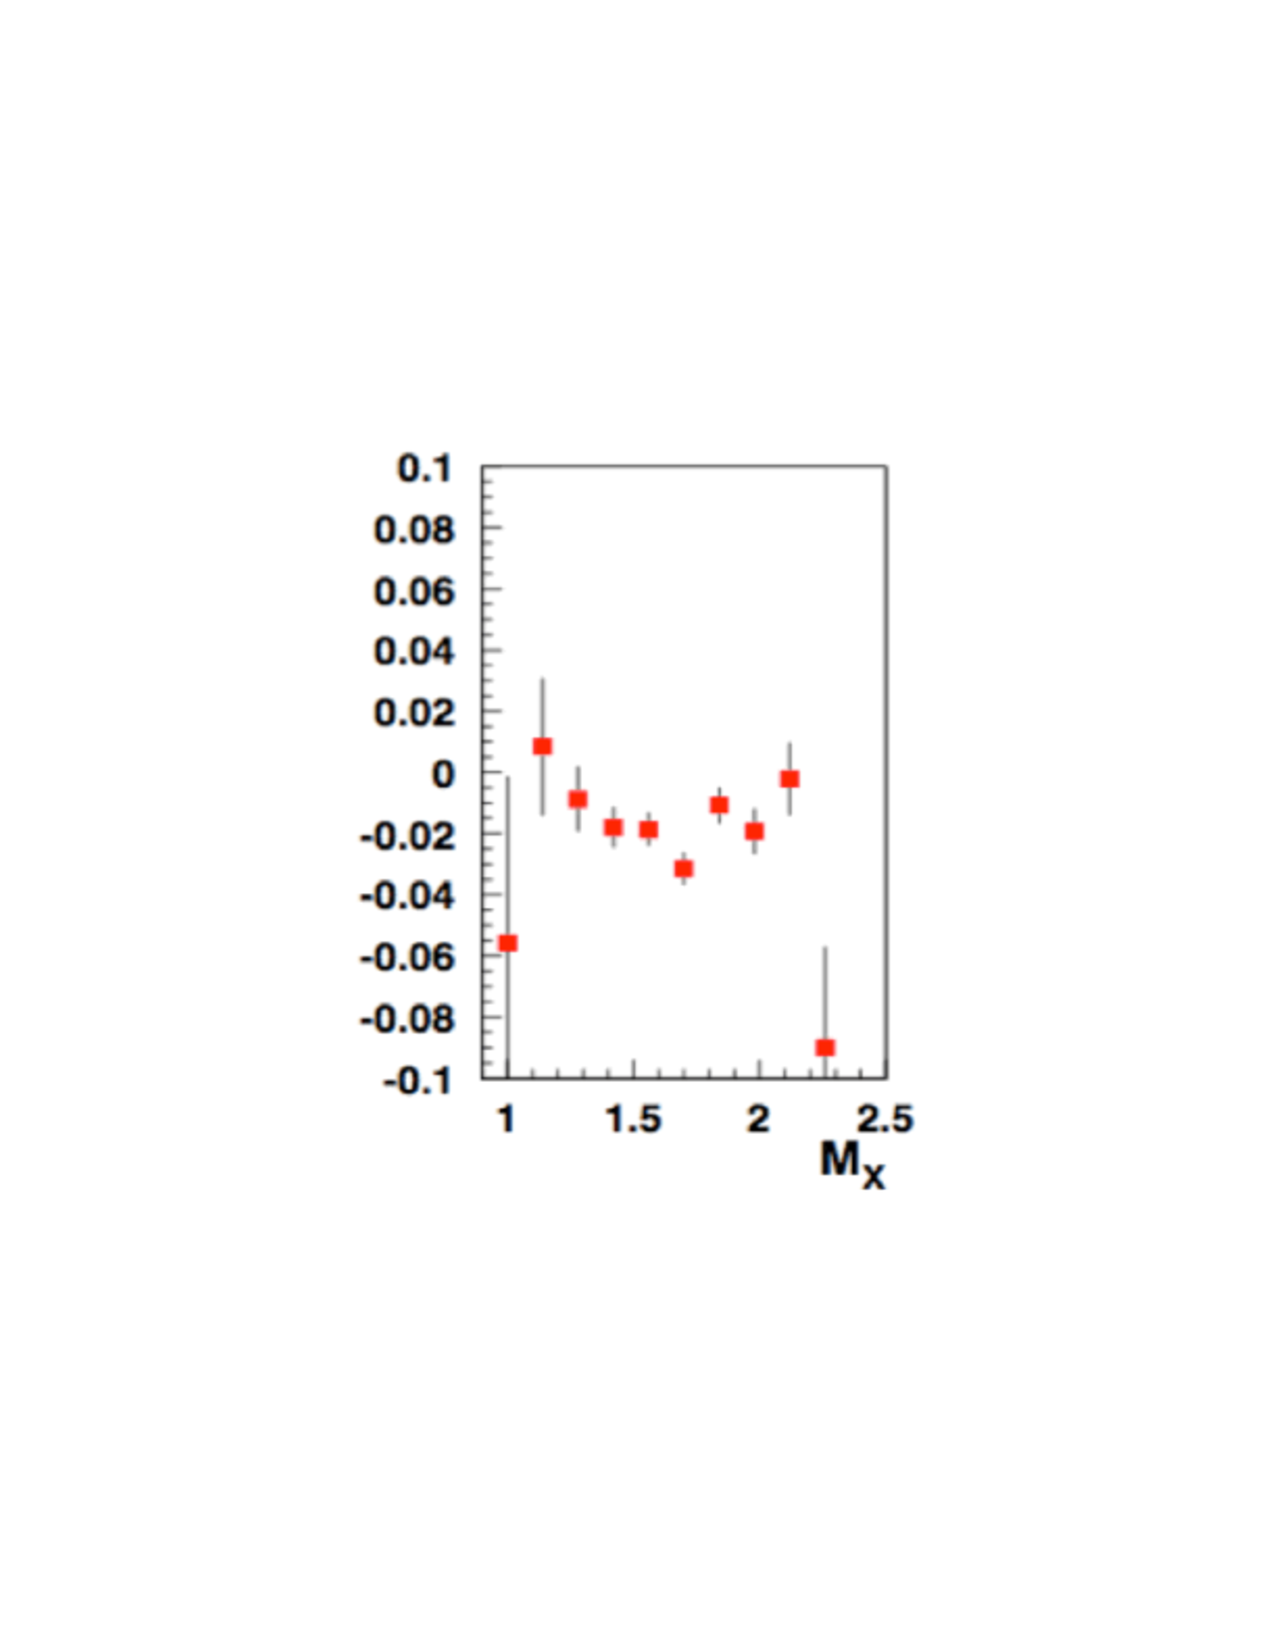
\includegraphics[width=8.1cm,height=7cm]{plots/alu-pi0mx.pdf}
\end{minipage}
   \caption{$A_{LU}$ dependence on missing mass of the $e\pi X$ system for $\pi^+$ (left), $\pi^-$ (middle) and  $\pi^0$ (right).}
 \label{fig:b2b-mx3}
 \end{figure} 



\section{Summary}

In conclusion, kinematic dependences of single spin asymmetries
are measured in a wide kinematic range at CLAS with polarized beam and unpolarized hydrogen  target. 
Significant single-spin asymmetries 
have been observed in back to back pion and proton
electroproduction.
Measurements of single-spin asymmetries indicate that spin-orbit correlations
may play an important role in description  of the structure of nucleon
in terms of elementary quarks and gluons going beyond the simple 
collinear partonic representation.

Within the canonical ranges of $x$, $Q^2$, $z$, $P_T$, $\phi$, 
$M_X$, a LO pQCD model of SIDIS, observed asymmetries may be interpreted in a framework
using fracture functions to describe the conditional probabilities of finding partons and hadronization functions
describing the fragmentation of the parton to final state hadrons in the current fragmentation.
Our results for $A_{LU}$, which are the first measurement of correlations between
target and current fragmentation regions, provide a new avenue for studies of the complex nucleon structure
in terms of quark and gluon degrees of freedom.
The dependence of the double spin asymmetry on the product of transverse momenta of two hadrons $P_{T1}P_{T2}$,  
suggest  that there is a trend in the
the dependence of the singl-spin asymmetry, consistent with expectations from theory.

A non-zero $A_{LU}$ in b2b SIDIS,  measured for the first time, indicate
that spin-orbit correlations  between hadrons
may be very significant.
The $x$-dependence of the the $A_{LU}^{\sin \phi}$ is consistent with asymmetry being large in the large-$\xbj$ region,
were the valence quark presence is very significant.

%\bibliographystyle{elsevier}
\bibliography{3dstructure}
\end{document}



